% =================================================================
% Systems Engineering (Wiley) article driver.
% Template: syseng.cls / ama.bst (modern 2026 Wiley Systems Engineering layout).
%
% TERMINOLOGY (vocabulary contract — use these terms consistently)
% ----------------------------------------------------------------
% Story: Every IOR generates a characteristic boundary fragment whose models are FSR(IOR).
%   On Φ_dyn, satisfaction is a Wymore homomorphism, and with buildability
%   that pairing is an implementable system design. Informally the implementability cotyledon
%   is the overlap of functionality and buildability; formally it is the pairing, not a
%   set intersection. Theorem 6.58 is identity-boundary only. The artifact worth keeping is
%   the fragment. The case study is pipelined streaming RLE on four components.
%
% Preferred terms:
%   DSYSTEM / discrete system — Wymore 5-tuple (S,I,O,δ,ρ); discrete clock;
%     state/IO may be infinite or real-valued.
%   Functionality Cotyledon CTL(IOR) / FSR(IOR) — set of systems satisfying IOR.
%   Input/Output Requirement IOR — 6-tuple (OLR, IR, ITR, OR, OTR, ER) specifying boundary intent.
%   Buildability Cotyledon CTL(TYR) / BSR(TYR) — designs (Z_b,SCR) buildable as resultants
%     RSY(SCR) across all valid SCRs with components from TYR.
%   Implementability Cotyledon CTL(IOR, TYR) / ISR(IOR, TYR) — implementable design pairs.
%   Functional design D_ref / D_f ∈ CTL(IOR); Z_ref is its system component.
%   Buildable resultant Z_b = RSY(SCR) ∈ CTL(TYR); mode Z_m ∈ SYSMO(Z_b).
%   Wymore system homomorphism / homomorphic image — surjective
%     h_S,h_I,h_O preserving transitions and readout.
%   Boundary temporal spec Φ_IOR; assertional functionality space AFSR(Φ_IOR) ≃ CTL(IOR).
%   Dynamics-encoding fragment Φ_dyn — G/X safety fragment compiled from Z_ref
%     (hom↔Φ_dyn bi-implication under surjective witness maps).
%   Assertional satisfaction — Z ⊨_IO Φ_IOR / Z ⊨_dyn Φ_dyn.
%   Operational time scale T (not "observation horizon").
% =================================================================

\documentclass[regular]{syseng}

% =================================================================
% Packages and macros for the Wiley Systems Engineering article (syseng.cls).
% Document class, authors, and abstract live in main.tex.
% =================================================================

\graphicspath{{./}{figures/}}
\usepackage[space]{grffile}
\usepackage{textcomp}
\usepackage{longtable}
\usepackage{colortbl}
\usepackage{tabularx}
\usepackage{multirow}
\usepackage{mathtools}
\usepackage{bm}
\usepackage{etoolbox}
\usepackage[english]{babel}
\usepackage{siunitx}
\usepackage{placeins}

\usepackage{tikz}
\usetikzlibrary{arrows,arrows.meta,positioning,shapes,shapes.geometric,fit,backgrounds,calc,automata}

% Compatibility aliases for natbib-style citation commands used in the text.
\providecommand{\citep}[1]{\cite{#1}}
\providecommand{\citet}[1]{\cite{#1}}
\providecommand{\citealt}[1]{\cite{#1}}

% Theorem and proof environments matching Wiley Systems Engineering style.
\newtheorem{theorem}{Theorem}
\newtheorem{lemma}[theorem]{Lemma}
\newtheorem{proposition}[theorem]{Proposition}
\newtheorem{corollary}[theorem]{Corollary}

\makeatletter
\def\@opargbegintheorem#1#2#3{\trivlist
   \item[\hskip \labelsep{\bfseries #1\ #2}]\textbf{(#3).}\ \itshape}
\makeatother

\newenvironment{proof}[1][Proof]{\begin{trivlist}
\item[\hskip \labelsep {\bfseries #1.}]}{\end{trivlist}}
\newenvironment{definition}[1][Definition]{\begin{trivlist}
\item[\hskip \labelsep {\bfseries #1.}]}{\end{trivlist}}
\newenvironment{example}[1][Example]{\begin{trivlist}
\item[\hskip \labelsep {\bfseries #1.}]}{\end{trivlist}}
\newenvironment{remark}[1][Remark]{\begin{trivlist}
\item[\hskip \labelsep {\bfseries #1.}]}{\end{trivlist}}

\newcommand{\qed}{\nobreak \ifvmode \relax \else
      \ifdim\lastskip<1.5em \hskip-\lastskip
      \hskip1.5em plus0em minus0.5em \fi \nobreak
      \vrule height0.75em width0.5em depth0.25em\fi}

% Table styling helpers.
\definecolor{tableheader}{HTML}{E6E6E6}
\newcolumntype{Y}{>{\raggedright\arraybackslash}X}
\newcolumntype{P}[1]{>{\centering\arraybackslash}p{#1}}
\newcolumntype{A}[1]{>{\raggedright\arraybackslash}p{#1}}
\newcolumntype{M}[1]{>{\raggedright\arraybackslash}m{#1}}
\newcommand{\headingfont}{}

% Lightweight stand-in for mini-heading macro.
\newcommand{\miniheading}[1]{%
  \par\vspace{4bp}\noindent\textbf{#1.}\space
}

% Safe figure include (optional assets).
\newcommand{\colfig}[2][]{%
  \IfFileExists{#2}{\includegraphics[width=\linewidth,#1]{#2}}{%
    \fbox{\parbox[b][1.5in][c]{\linewidth}{\centering \textit{Missing figure: }#2}}}%
}

\newif\iflatexml\latexmlfalse
\providecommand{\tightlist}{\setlength{\itemsep}{0pt}\setlength{\parskip}{0pt}}%

\AtBeginDocument{\DeclareGraphicsExtensions{.pdf,.PDF,.eps,.EPS,.png,.PNG,.tif,.TIF,.jpg,.JPG,.jpeg,.JPEG}}


\pubyear{2026}
\volume{0}
\doi{10.1002/sys.00000}
\received{TBD October 2026}
\revised{TBD 2026}
\accepted{TBD 2026}
\correspondence{Nicholas McKibben, Department of Systems and Industrial Engineering, University of Arizona, Tucson, AZ 85721, USA (\href{mailto:mckib2@arizona.edu}{mckib2@arizona.edu})}
\funding{None}

\keywords{Tricotyledon Theory of System Design (T3SD) \kwsep Linear Temporal Logic (LTL) \kwsep formal verification \kwsep Model-Based Systems Engineering (MBSE) \kwsep system modes}

\title{Reinterpreting the Functionality Cotyledon: Temporal Logic for T3SD}

\author{%
  Nicholas McKibben\affilmark{1} \authorsep
  Larry Head\affilmark{1} \authorsep
  Alejandro Salado\affilmark{1}%
}

\affiliations{%
  \affilnum{1}Department of Systems and Industrial Engineering, University of Arizona, Tucson, AZ, USA%
}

\abstract{%
In Wymore's Tricotyledon Theory of System Design (T3SD), an input/output requirement (IOR) defines the functionality cotyledon of systems satisfying desired boundary trajectories, while a technology catalog defines the buildability cotyledon of coupled architectures assembled across valid system coupling recipes. Certifying implementability requires isolating an operational mode of a buildable resultant and exhibiting a surjective homomorphism that maps onto a functional design, a manual process that becomes arduous for coupled systems and lacks automated tooling. This paper develops a correspondence between T3SD and temporal logic to enable automated model checking within Wymore's framework. First, we prove that every IOR is isomorphic to an assertional boundary specification in temporal logic. Second, we show that certifying a buildable system mode reduces to checking temporal specifications directly, avoiding manual homomorphism construction while preserving conformance across state re-encodings and component elaborations. Because buildable components are generally finite-state, Linear Temporal Logic (LTL) model checking over their operational modes is decidable and automated, which we demonstrate by verifying a coupled streaming run-length encoder across finite-capacity component catalogs.%
}

\begin{document}

\maketitle

% ----- Main body (in order) -----
\section{Introduction}
\label{sec:introduction}

Wymore's Tricotyledon Theory of System Design (T3SD) provides a rigorous mathematical foundation for Model-Based Systems Engineering (MBSE) by separating what a system must do at its external boundary from how it can be constructed out of available components \citep{Wymore1993,salado2019wymore,salado2019mbse}. An Input/Output Requirement ($IOR$) specifies admissible input trajectories and their eligible output trajectories over an operational horizon, generating the \emph{functionality cotyledon} $\mathrm{CTL}(IOR)=\mathrm{FSR}(IOR)$---a space of functional system designs that is provably either empty (if the requirement violates causality) or infinite \citep{Wymore1993}. Independently, a technology ($TYR$) cataloging available hardware or software components and a System Coupling Recipe ($SCR$) wiring their ports generate the \emph{buildability cotyledon} $\mathrm{CTL}(TYR)=\mathrm{BSR}(TYR)$, whose members are coupled resultant systems $Z_b=\mathrm{RSY}(SCR)$.

Connecting these two design spaces is the central verification problem of T3SD. A candidate architecture belongs to the \emph{implementability cotyledon} $\mathrm{CTL}(IOR,TYR)=\mathrm{ISR}(IOR,TYR)$ when a buildable resultant $Z_b\in\mathrm{CTL}(TYR)$ \emph{implements} a functional system design $Z_f\in\mathrm{CTL}(IOR)$ \citep{Wymore1993}. Because a physical or digital build typically contains internal clock phases, initialization states, diagnostic registers, or unused capacity that are not part of the abstract functional model, Wymore defines implementation in two stages: one first isolates a \emph{system mode} $Z_m\in\mathrm{SYSMO}(Z_b)$ representing the operational regime of the build, and then exhibits a surjective, transition- and readout-preserving \emph{system homomorphism} $h=(h_S,h_I,h_O)$ from $Z_m$ onto $Z_f$.

While mathematically complete, this constructive workflow faces a severe practical bottleneck. First, $\mathrm{CTL}(IOR)$ is infinite when nonempty, forcing the engineer to select a particular reference machine $Z_{\mathrm{ref}}\in\mathrm{CTL}(IOR)$ and manually construct a state-space mapping $h_S:S_m\to S_{\mathrm{ref}}$ from the coupled product state space of $Z_m$ onto $Z_{\mathrm{ref}}$. Second, deciding whether a surjective homomorphism exists between finite transition systems is NP-hard in general \citep{HellNesetril1990,BodirskyKaraMartin2012}, and even small representation changes---such as flipping a phase bit or adding a diagnostic counter to a component---require reconstructing and re-proving the homomorphism maps by hand. Third, because T3SD has remained a specialized systems engineering theory, it has not developed the mature ecosystem of automated solvers and model checkers that computer science built for temporal logic \citep{Pnueli1977,BaierKatoen2008}.

This paper resolves that bottleneck by establishing a formal bridge between T3SD and temporal logic. Rather than replacing Wymore's cotyledons, we show that temporal logic provides an exact, tool-supported language for specifying the functionality cotyledon and automatically certifying homomorphic implementation of system modes. Specifically, this paper makes four contributions:
\begin{enumerate}
    \item \textbf{Isomorphism between Wymorian $IOR$s and boundary temporal specifications.} For every Wymorian $IOR$, we construct a characteristic boundary temporal specification $\Phi_{IOR}$ whose trajectory satisfaction predicate is identical to Wymore's $\mathrm{SatisfiesIOR}$, yielding a canonical bijection $\mathrm{AFSR}(\Phi_{IOR})\simeq\mathrm{FSR}(IOR)$ between the assertional functionality space and the functionality cotyledon.
    \item \textbf{Direct mode-to-$IOR$ verification without manual homomorphisms.} Using Wymore's requirement-preservation theorem (Theorem~6.58) alongside a compiled dynamics fragment $\Phi_{\mathrm{dyn}}(Z_{\mathrm{ref}})$, we prove that a system mode $Z_m\in\mathrm{SYSMO}(Z_b)$ admits an identity-boundary homomorphism onto a functional system in $\mathrm{CTL}(IOR)$ if and only if $Z_m\models\Phi_{IOR}$ directly. When a specific reference architecture $Z_{\mathrm{ref}}\in\mathrm{CTL}(IOR)$ is chosen, $Z_m\models_{\mathrm{dyn}}\Phi_{\mathrm{dyn}}(Z_{\mathrm{ref}})$ is necessary and sufficient for $Z_{\mathrm{ref}}$ to be a homomorphic image of $Z_m$, placing $(Z_{\mathrm{ref}},Z_b)$ in the implementability cotyledon $\mathrm{CTL}(IOR,TYR)$.
    \item \textbf{Decidable LTL model checking for finite buildable modes and invariance across refactoring.} Because real-world buildable components in $TYR$ are finite-state machines, any coupled resultant $Z_b=\mathrm{RSY}(SCR)$ and any operational mode $Z_m\in\mathrm{SYSMO}(Z_b)$ is a finite transition system. When $\Phi_{IOR}$ is expressed in Linear Temporal Logic (LTL), verifying $Z_m\models\Phi_{IOR}$ is decidable and fully automated via standard LTL model checking \citep{BaierKatoen2008}, and conformance is preserved under state re-encoding, port relabeling, and componentwise elaboration.
    \item \textbf{End-to-end infinite-to-finite case study on a coupled streaming Run-Length Encoder (RLE).} We develop a four-component coupled machine (tape, sense/act head, state register, and instruction table) starting from an idealized infinite-tape / unbounded-count specification in $\mathrm{CTL}(IOR_\infty)$ and systematically refining it to a finite-tape buildable resultant $Z_{b,N}=\mathrm{RSY}(SCR_N)\in\mathrm{CTL}(TYR_N)$. An automated LTL checker verifies the active-phase system mode across nominal caps, phase re-encodings, and register instrumentation while pinpointing the exact violated temporal clauses in faulty variants.
\end{enumerate}

The remainder of the paper is organized as follows. Section~\ref{sec:background} reviews the three cotyledons, system modes, homomorphisms, and temporal logic operators in accessible systems engineering terms. Section~\ref{sec:methodology} establishes the boundary $IOR$ isomorphism, the mode-to-$IOR$ implementability theorems, and the invariance and compositional lifting properties. Section~\ref{sec:case-study} presents the streaming RLE case study from its infinite-count formulation through its finite-tape refinement and automated LTL verification. Section~\ref{sec:discussion} discusses expressivity, pipeline timing, and systems engineering implications, and Section~\ref{sec:conclusions} concludes.

\section{Background} \label{sec:background}

\subsection{Discrete Systems and Cotyledons}
In Wymore's framework, a discrete system (denoted $\mathrm{DSYSTEM}$ in \citet{Wymore1993}) is a deterministic Moore-type state machine defined by a quintuple $Z=(S,I,O,\delta,\rho)$ consisting of a nonempty state set $S$, an input alphabet $I$, an output alphabet $O$, a next-state transition function $\delta:S\times I\to S$, and a state readout function $\rho:S\to O$. Here ``discrete'' refers to the discrete time scale $T=\mathbb{N}$; the state and port sets $S$, $I$, and $O$ may be either finite (as in physical digital hardware) or countably infinite (as in idealized mathematical specifications with, e.g., unbounded counters). Given an initial state $s_0\in S$ and an input trajectory $f:T\to I$, iterating $\delta$ from $s_0$ generates a unique state trajectory $g(t)$ (Wymore's $\mathrm{STZ}(Z,s_0,f)(t)$) and a corresponding boundary output trajectory $y(t)=\rho(g(t))$ (Wymore's $\mathrm{OTZ}(Z,s_0,f)(t)$). Because $\rho$ is a function of the current state $g(t)$ alone, every Wymorian discrete system obeys Moore causality: an external input $f(t)$ arriving at tick $t$ first affects the next state $g(t+1)=\delta(g(t),f(t))$ and can therefore influence the boundary output no earlier than tick $t+1$.

T3SD organizes a system design problem around three mathematical spaces, called \emph{cotyledons} after their leaf-shaped depiction in Wymore's diagrams \citep{Wymore1993}:
\begin{enumerate}
    \item \textbf{Functionality Cotyledon $\mathrm{CTL}(IOR)$.} An input/output requirement is a 6-tuple $IOR=(OLR,IR,ITR,OR,OTR,ER)$, where $OLR$ specifies the operational length (defining the required time scale $T_{IOR}\subseteq\mathbb{N}$), $IR$ and $OR$ are the boundary input and output alphabets, $ITR\subseteq IR^T$ and $OTR\subseteq OR^T$ are the sets of admissible input and output trajectories, and $ER\subseteq ITR\times OTR$ is the eligibility relation pairing each admissible input trajectory $f\in ITR$ with its set of acceptable output trajectories $ER(f)\subseteq OTR$. A \emph{functional system design} $D_f=(Z_f,s_0,T_f)\in\mathrm{CTL}(IOR)$ (the Functionality Space Requirement, $\mathrm{FSR}(IOR)$) packages a discrete system $Z_f$ on boundary alphabets $(IR,OR)$, a designated initial state $s_0$, and a nonempty observation horizon $T_f\subseteq T_{IOR}$ such that for every $f\in ITR$ (and any input extension agreeing with $f$ on $T_{IOR}$), the output trajectory generated by $Z_f$ from $s_0$ agrees on $T_f$ with some eligible trajectory $g\in ER(f)$. Wymore's shows that $\mathrm{CTL}(IOR)$ is either empty (when $IOR$ violates Moore causality) or infinite, because once a single realizing state machine exists, any state re-encoding or state-space elaboration yields another distinct member of $\mathrm{CTL}(IOR)$ (see Theorem~6.64 in \citep{Wymore1993}).
    \item \textbf{Buildability Cotyledon $\mathrm{CTL}(TYR)$.} A technology $TYR$ is a nonempty catalog of available discrete component systems (such as hardware registers, sensors, clocks, or software modules). A System Coupling Recipe $SCR=(VSCR,CSCR)$ specifies a vector $VSCR$ of component systems together with an internal port-to-port feedback and feedforward wiring relation $CSCR$. When every component in $VSCR$ is selected from the catalog $TYR$, synchronous composition of the wired components produces a unique coupled \emph{resultant} discrete system $Z_b=\mathrm{RSY}(SCR)$ whose external boundary inputs and outputs are the unconnected input and output ports of the recipe (denoted $\mathrm{UISCR}(SCR)$ and $\mathrm{UOSCR}(SCR)$ in \citet{Wymore1993}). The buildability cotyledon $\mathrm{CTL}(TYR)$ (the Buildability Space Requirement, $\mathrm{BSR}(TYR)$) consists of all such buildable designs $D_b=(SCR,Z_b)$ constructible from $TYR$.
    \item \textbf{Implementability Cotyledon $\mathrm{CTL}(IOR,TYR)$.} Informally, we may uderstand the implementability cotyledon as the intersection between functionality and buildability, i.e., those systems that both satisfy the input/output requirement and are constructible from the available technology. Formally, because functional designs specify abstract boundary behavior whereas buildable designs specify coupled component architectures with potentially different state spaces and port structures, $\mathrm{CTL}(IOR,TYR)$ (the Implementability Space Requirement, $\mathrm{ISR}(IOR,TYR)$) is defined as the set of pairs $(D_f,D_b)\in\mathrm{CTL}(IOR)\times\mathrm{CTL}(TYR)$ linked by Wymore's \emph{implementation} relation ($\mathrm{IMPSY}$, Definition~5.71) \citep{Wymore1993}.
\end{enumerate}
Throughout this paper, when the initial state $s_0$, observation horizon $T$, and coupling recipe $SCR$ are clear from context, we identify a functional design $D_f=(Z_f,s_0,T)$ with its underlying system $Z_f\in\mathrm{CTL}(IOR)$ and a buildable design $D_b=(SCR,Z_b)$ with its coupled resultant $Z_b=\mathrm{RSY}(SCR)\in\mathrm{CTL}(TYR)$, writing implementable pairs in $\mathrm{CTL}(IOR,TYR)$ as $(D_f,Z_b)$.

\subsection{System Modes, Homomorphisms, and Implementation}
\label{sec:background-modes-hom}
We would rarely expect a buildable resultant $Z_b=\mathrm{RSY}(SCR)$ to satisfy an abstract functional model $Z_f\in\mathrm{CTL}(IOR)$ by direct state-space equality, as at the very least, the two systems will almost certainly have different state spaces.  In practice, a coupled architecture contains implementation details that do not appear in an idealized functional specification: multi-phase internal clocks, pipeline latches, post-reset initialization states, diagnostic registers, or unused port encodings. Conversely, an idealized functional model may be stated over an infinite state space (such as an unbounded counter), whereas any physical machine operates within a bounded hardware capacity.

Wymore introduces two concepts to relate buildable resultants and functional models:
\begin{itemize}
    \item \textbf{System Mode ($\mathrm{SYSMO}$, see Definition~5.6 in \citet{Wymore1993}).} A discrete system $Z_m=(S_m,I_m,O_m,\delta_m,\rho_m)$ is a \emph{system mode} of a buildable system $Z_b=(S_b,I_b,O_b,\delta_b,\rho_b)$, written $Z_m\in\mathrm{SYSMO}(Z_b)$, if $Z_m$ embeds into $Z_b$ via injective maps on states, inputs, and outputs such that each step of $Z_m$ corresponds to a well-defined trajectory segment of $Z_b$ within an invariant operational regime (for example, restricting $Z_b$ to its reachable post-reset states, an active clock phase, or a bounded operating envelope). Every system is trivially a mode of itself via its primary self-mode.
    \item \textbf{System Homomorphism ($\mathrm{HIMSY}$, see Definition~4.3 in \citet{Wymore1993}).} A functional system $Z_f=(S_f,I_f,O_f,\delta_f,\rho_f)$ is a \emph{homomorphic image} of $Z_m$ (written $Z_f\in\mathrm{HIMSY}(Z_m)$) if there exist \emph{surjective} maps $h_S:S_m\twoheadrightarrow S_f$, $h_I:I_m\twoheadrightarrow I_f$, and $h_O:O_m\twoheadrightarrow O_f$ (denoted $\mathrm{HS}$, $\mathrm{HI}$, and $\mathrm{HO}$ in \citet{Wymore1993}) that commute with state transitions and readouts at every state $x\in S_m$ and input $p\in I_m$:
    \begin{equation}
        h_S(\delta_m(x,p)) = \delta_f(h_S(x),h_I(p)), \qquad h_O(\rho_m(x)) = \rho_f(h_S(x)).
        \label{eq:wymore-hom-def}
    \end{equation}
\end{itemize}
By Definition~5.71 in \citet{Wymore1993}, a buildable resultant $Z_b$ \emph{implements} a functional system $Z_f$ (written $Z_f\in\mathrm{IMPSY}(Z_b)$) if and only if $Z_f$ is a homomorphic image of at least one system mode $Z_m\in\mathrm{SYSMO}(Z_b)$. Wymore's Theorem~6.58 further establishes that when $Z_m$ and $Z_f$ share the boundary alphabets $(IR,OR)$ with identity port maps ($h_I=\mathrm{id}_{IR}$, $h_O=\mathrm{id}_{OR}$), any homomorphism $h_S:S_m\twoheadrightarrow S_f$ preserves $IOR$ satisfaction across corresponding initial states:
\begin{equation}
    \mathrm{SatisfiesIOR}(Z_m,IOR,s_0,T) \Longleftrightarrow \mathrm{SatisfiesIOR}(Z_f,IOR,h_S(s_0),T).
    \label{eq:thm-658-preview}
\end{equation}

\miniheading{Notation}
Table~\ref{tab:notation} summarizes Wymore's textbook nomenclature \citep{Wymore1993} alongside the standard mathematical notation used throughout this paper.

\begin{table*}[t]
\caption{Correspondence between Wymore's T3SD terminology \citep{Wymore1993} and the mathematical notation used in this paper.}
\label{tab:notation}
\renewcommand{\arraystretch}{1.25}
\footnotesize
\begin{tabularx}{\textwidth}{@{}A{0.25\textwidth} A{0.35\textwidth} >{\raggedright\arraybackslash}X@{}}
    \toprule
    \textbf{Concept} & \textbf{Wymore (T3SD)} & \textbf{Notation in This Paper} \\
    \midrule
    Discrete system 5-tuple & $\mathrm{DSYSTEM}\ (SZ, IZ, OZ, \mathrm{NZ}, \mathrm{RZ})$ & $Z = (S, I, O, \delta, \rho)$ \\
    State / output trajectories & $\mathrm{STZ}(Z,s_0,f)(t),\ \mathrm{OTZ}(Z,s_0,f)(t)$ & $g(t),\ y(t)=\rho(g(t))$ \\
    Input/Output Requirement & $\mathrm{IOR} = (\mathrm{OLR},\mathrm{IR},\mathrm{ITR},\mathrm{OR},\mathrm{OTR},\mathrm{ER})$ & $IOR = (OLR, IR, ITR, OR, OTR, ER)$ \\
    Functionality Cotyledon & $\mathrm{CTL}(\mathrm{IOR}) = \mathrm{FSR}(\mathrm{IOR})$ & $\mathrm{CTL}(IOR) = \mathrm{FSR}(IOR)$ \\
    Buildability Cotyledon & $\mathrm{CTL}(\mathrm{TYR}) = \mathrm{BSR}(\mathrm{TYR})$ & $\mathrm{CTL}(TYR) = \mathrm{BSR}(TYR)$ \\
    Implementability Cotyledon & $\mathrm{CTL}(\mathrm{IOR}, \mathrm{TYR}) = \mathrm{ISR}(\mathrm{IOR},\mathrm{TYR})$ & $\mathrm{CTL}(IOR, TYR) = \mathrm{ISR}(IOR, TYR)$ \\
    Coupling recipe \& resultant & $\mathrm{SCR} = (\mathrm{VSCR}, \mathrm{CSCR}),\ \mathrm{RSY}(\mathrm{SCR})$ & $SCR = (VSCR, CSCR),\ Z_b = \mathrm{RSY}(SCR)$ \\
    System modes of $Z_b$ & $\mathrm{SYSMO}(Z_b)$ & $Z_m \in \mathrm{SYSMO}(Z_b)$ \\
    Homomorphic image / maps & $Z_f \in \mathrm{HIMSY}(Z_m)$ via $(\mathrm{HS},\mathrm{HI},\mathrm{HO})$ & $h = (h_S, h_I, h_O) : Z_m \twoheadrightarrow Z_f$ \\
    Implementation relation & $Z_f \in \mathrm{IMPSY}(Z_b)$ & $\exists Z_m \in \mathrm{SYSMO}(Z_b),\ h : Z_m \twoheadrightarrow Z_f$ \\
    Temporal specifications & --- & $Z_m\models_{IO}\Phi_{IOR}$ (boundary),\ $Z_m\models_{\mathrm{dyn}}\Phi_{\mathrm{dyn}}(Z_{\mathrm{ref}})$ (dynamics) \\
    \bottomrule
\end{tabularx}
\end{table*}

\subsection{Temporal Logics and Model Checking}
\label{sec:background-ltl}
Linear Temporal Logic (LTL) and its first-order extensions provide a formal language for expressing properties of time-indexed trajectories \citep{Pnueli1977,MannaPnueli1995,BaierKatoen2008,VardiWolper1986,Thomas1990}. Rather than specifying desired behavior by constructing a concrete state set and transition table, a temporal formula characterizes the admissible infinite or finite traces directly using Boolean connectives ($\wedge,\vee,\neg,\rightarrow$) and temporal modalities such as $G\,\varphi$ (``always $\varphi$'') and $X\,\varphi$ (``at the next tick, $\varphi$''), summarized in Table~\ref{tab:ltl-operators}.

\begin{table}[t]
\caption{Core temporal logic operators used to express boundary requirements $\Phi_{IOR}$ and compiled dynamics $\Phi_{\mathrm{dyn}}$.}
\label{tab:ltl-operators}
\renewcommand{\arraystretch}{1.2}
\footnotesize
\setlength{\tabcolsep}{4pt}
\begin{tabularx}{\columnwidth}{@{}l l >{\raggedright\arraybackslash}p{0.28\columnwidth} >{\raggedright\arraybackslash}X@{}}
    \toprule
    \textbf{Op.} & \textbf{Name} & \textbf{Role in T3SD} & \textbf{Semantics at Tick $t$} \\
    \midrule
    $G\,\varphi$ & always & Global invariant & $\varphi$ holds at all $\tau \ge t$ \\
    $X\,\varphi$ & next & 1-step delay & $\varphi$ holds at $t+1$ \\
    $\varphi \rightarrow \psi$ & implies & Guarded step & If $\varphi$ at $t$, then $\psi$ at $t$ \\
    $\varphi \wedge \psi$ & and & Joint guard & Both $\varphi$ and $\psi$ hold at $t$ \\
    $F\,\varphi$ & eventually & Attainment & $\varphi$ holds at some $\tau \ge t$ \\
    \bottomrule
\end{tabularx}
\end{table}

When a discrete system $Z_m$ has finite state, input, and output sets, its execution defines a finite Kripke structure whose paths are infinite sequences of $(s(t),i(t),y(t))$ triples. Deciding whether every run of a finite-state system satisfies an LTL formula ($Z_m\models\varphi$) is PSPACE-complete \citep{SistlaClarke1985} and supported by established explicit-state, symbolic binary decision diagram (BDD), and SAT/SMT-based model checkers \citep{BurchClarkeMcMillanDill1992,BiereCimattiClarkeZhu1999,BaierKatoen2008,deMouraZ32008}.

\subsection{Related Work}
\label{sec:related-work}
Several lines of research across systems engineering, formal verification, and computational complexity inform the approach developed in this paper.

Within the MBSE literature, recent work has revisited Wymore's T3SD to provide a rigorous systems-theoretic foundation for modern modeling practices. Salado and Wach \citep{salado2019wymore,salado2019mbse} demonstrated how Wymorian input/output requirements can ground True Model-Based Requirements (TMBR) in SysML without conflating problem-space boundary requirements with internal solution architectures, while Wach et al.\ \citep{wach2021devs} connected Wymore's discrete systems to Discrete Event System Specification (DEVS) \citep{ZeiglerPraehoferKim2000}. Mainstream SysML/UML practice, however, lacks a native mathematical notion of homomorphism between problem-space boundary requirements and coupled buildable resultants, so architectural verification often remains descriptive or else exports the entire diagram into an external semantic substrate such as Petri nets or transition systems \citep{Jensen1997,ZeiglerPraehoferKim2000}.  T3SD-oriented modernization efforts preserve the separation between the functionality and buildability cotyledons; however, they still rely on Wymore's classical constructive $\mathrm{IMPSY}$ definitions when certifying that a coupled architecture implements a requirement. The present paper retains Wymore's coupling algebra $\mathrm{RSY}$ and system modes $\mathrm{SYSMO}$ and automates where possible the implementability check through temporal specifications $\Phi_{IOR}$ and $\Phi_{\mathrm{dyn}}$.

Contract-based design and interface theories provide a complementary vocabulary for boundary requirements.  Assume/guarantee contracts and interface automata typically partition concerns into environmental assumptions and system guarantees \citep{BenvenisteEtAl2018,deAlfaroHenzinger2001}. A Wymorian $IOR$, by contrast, packages admissible input trajectories $ITR$ together with an eligibility relation $ER\subseteq ITR\times OTR$ that pairs each admissible input with its acceptable outputs. Expressing that eligibility relation as a boundary temporal specification $\Phi_{IOR}$ makes $IOR$ satisfaction tool-checkable in the spirit of contract-style boundary verification, while retaining Wymore's Moore causality at the readout boundary; we do not identify $IOR$s with assume/guarantee contracts, but rather note that $\Phi_{IOR}$ supplies a temporally executable account of the same trajectory-level intent that contracts address at interfaces.

In formal methods and concurrency theory, temporal logic safety fragments have long been used to characterize step-local transition invariants \citep{Sistla1994,MannaPnueli1995}, and characteristic-formula constructions encode operational state machines into modal or temporal logic formulas up to simulation or bisimulation equivalence \citep{Milner1989,GrafSifakis1986,SteffenIngolfsdottir1994,AcetoEtAl2012}. Those constructions typically target action-labeled transition systems and often rely on the modal calculi to characterize branching or weak behavioral equivalences. Algebraically, Wymore's surjective system homomorphism corresponds to a bounded morphism on deterministic Moore coalgebras \citep{Rutten2000,BlackburnDeRijkeVenema2001}. T3SD systems, however, are deterministic Moore machines with synchronous port-based coupling ($\mathrm{RSY}$) and operational modes ($\mathrm{SYSMO}$) that preserve step-local autonomous behavior. Consequently, the dynamics fragment $\Phi_{\mathrm{dyn}}$ is intentionally a step-local $G$/$X$ safety fragment that mirrors Wymore's static homomorphism axioms (see Definition~4.3 in \citet{Wymore1993}), rather than a full characteristic formula for branching bisimulation. However, prior characteristic-formula results do not, out of the box, connect trajectory-based $IOR$s, system modes, and coupling recipes within the tricotyledon framework.  This is a gap that this paper addresses.

Finally, classical refinement theories and combinatorial complexity delimit what lock-step T3SD verification can and cannot claim. Refinement mappings and hierarchical I/O automata permit internal stuttering or silent steps between corresponding observable transitions \citep{AbadiLamport1991,LynchTuttle1987,Lamport2002}. Wymore's implementation relation instead equates one tick of the buildable mode with one tick of the functional design: intermediate execution artifacts are handled by first isolating an operational system mode $Z_m\in\mathrm{SYSMO}(Z_b)$ and then exhibiting a surjective step-synchronous homomorphism onto $Z_f$. The compiled fragment $\Phi_{\mathrm{dyn}}$, which retains the next-step operator $X$, is therefore the exact temporal counterpart of classical T3SD.  Multi-rate and stuttering relaxations are not considered in this work. Deciding whether a surjective homomorphism exists between finite relational structures or transition systems is NP-hard in general \citep{HellNesetril1990,BodirskyKaraMartin2012}, and maintaining an explicit state-space projection $h_S:S_m\twoheadrightarrow S_f$ is fragile under architectural revision. By translating $IOR$s and reference dynamics into temporal specifications evaluated over finite buildable system modes, our work replaces manual homomorphism construction with decidable LTL and SAT-based checking \citep{SistlaClarke1985,BaierKatoen2008}.

\section{Methodology} \label{sec:methodology}

\subsection{Reinterpreting the Functionality Cotyledon}
Figure~\ref{fig:cotyledons-bridge} illustrates the structural relationship between Wymore's three cotyledons and the temporal logic correspondence developed in this section. On the left, an input/output requirement $IOR$ generates the functionality cotyledon $\mathrm{CTL}(IOR)=\mathrm{FSR}(IOR)$, from which a functional system design $D_f=(Z_f,s_0,T)$ may be selected. On the right, a technology catalog $TYR$ and coupling recipe $SCR$ generate a coupled buildable resultant $Z_b=\mathrm{RSY}(SCR)\in\mathrm{CTL}(TYR)$, from which an operational system mode $Z_m\in\mathrm{SYSMO}(Z_b)$ is isolated.

\begin{figure*}[t]
  \centering
  \resizebox{0.94\textwidth}{!}{%
  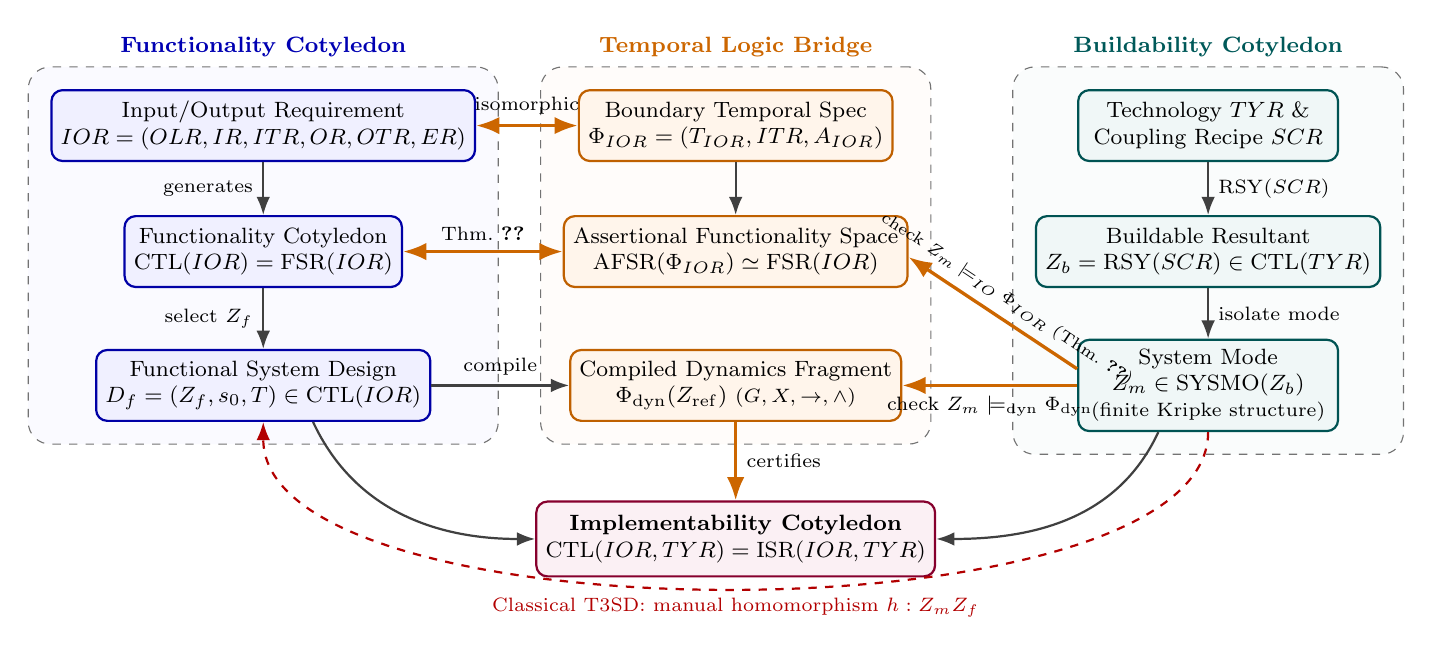
\begin{tikzpicture}[auto, >=Latex, thick,
    cotyledon/.style={draw=black!55, dashed, rounded corners=8pt, inner sep=8pt},
    funcbox/.style={draw=blue!65!black, fill=blue!6, rectangle, rounded corners=4pt, minimum width=3.3cm, minimum height=0.9cm, align=center, font=\footnotesize},
    buildbox/.style={draw=teal!65!black, fill=teal!6, rectangle, rounded corners=4pt, minimum width=3.3cm, minimum height=0.9cm, align=center, font=\footnotesize},
    logicbox/.style={draw=orange!75!black, fill=orange!8, rectangle, rounded corners=4pt, minimum width=3.4cm, minimum height=0.9cm, align=center, font=\footnotesize},
    isrbox/.style={draw=purple!70!black, fill=purple!6, rectangle, rounded corners=4pt, minimum width=3.8cm, minimum height=0.95cm, align=center, font=\footnotesize\bfseries},
    arrow/.style={->, >=Latex, thick, draw=black!75},
    homarrow/.style={->, >=Latex, dashed, thick, draw=red!70!black},
    ltlarrow/.style={->, >=Latex, very thick, draw=orange!80!black}
  ]
    % Left: Functionality Cotyledon
    \node (ior) [funcbox] at (0, 2.7) {Input/Output Requirement\\$IOR=(OLR,IR,ITR,OR,OTR,ER)$};
    \node (fsr) [funcbox] at (0, 1.1) {Functionality Cotyledon\\$\mathrm{CTL}(IOR)=\mathrm{FSR}(IOR)$};
    \node (dref) [funcbox] at (0, -0.6) {Functional System Design\\$D_f=(Z_f,s_0,T)\in\mathrm{CTL}(IOR)$};

    % Center: Temporal Logic & Implementability
    \node (phiIOR) [logicbox] at (6.0, 2.7) {Boundary Temporal Spec\\$\Phi_{IOR}=(T_{IOR},ITR,A_{IOR})$};
    \node (afsr) [logicbox] at (6.0, 1.1) {Assertional Functionality Space\\$\mathrm{AFSR}(\Phi_{IOR})\simeq\mathrm{FSR}(IOR)$};
    \node (phiDyn) [logicbox] at (6.0, -0.6) {Compiled Dynamics Fragment\\$\Phi_{\mathrm{dyn}}(Z_{\mathrm{ref}})$ {\scriptsize ($G,X,\rightarrow,\wedge$)}};
    \node (isr) [isrbox] at (6.0, -2.55) {Implementability Cotyledon\\$\mathrm{CTL}(IOR,TYR)=\mathrm{ISR}(IOR,TYR)$};

    % Right: Buildability Cotyledon
    \node (tyr) [buildbox] at (12.0, 2.7) {Technology $TYR$ \&\\Coupling Recipe $SCR$};
    \node (bsr) [buildbox] at (12.0, 1.1) {Buildable Resultant\\$Z_b=\mathrm{RSY}(SCR)\in\mathrm{CTL}(TYR)$};
    \node (mode) [buildbox] at (12.0, -0.6) {System Mode\\$Z_m\in\mathrm{SYSMO}(Z_b)$\\{\scriptsize (finite Kripke structure)}};

    % Cotyledon Group Boxes
    \begin{scope}[on background layer]
      \node[cotyledon, fill=blue!2, fit=(ior)(fsr)(dref), label={[font=\footnotesize\bfseries, text=blue!70!black]above:Functionality Cotyledon}] {};
      \node[cotyledon, fill=orange!2, fit=(phiIOR)(afsr)(phiDyn), label={[font=\footnotesize\bfseries, text=orange!80!black]above:Temporal Logic Bridge}] {};
      \node[cotyledon, fill=teal!2, fit=(tyr)(bsr)(mode), label={[font=\footnotesize\bfseries, text=teal!70!black]above:Buildability Cotyledon}] {};
    \end{scope}

    % Vertical / internal arrows
    \draw[arrow] (ior) -- node[left, font=\scriptsize] {generates} (fsr);
    \draw[arrow] (fsr) -- node[left, font=\scriptsize] {select $Z_f$} (dref);
    \draw[arrow] (tyr) -- node[right, font=\scriptsize] {$\mathrm{RSY}(SCR)$} (bsr);
    \draw[arrow] (bsr) -- node[right, font=\scriptsize] {isolate mode} (mode);

    % Horizontal bridge arrows
    \draw[ltlarrow, <->] (ior) -- node[above, font=\scriptsize] {isomorphic} (phiIOR);
    \draw[ltlarrow, <->] (fsr) -- node[above, font=\scriptsize] {Thm.~\ref{thm:boundary-characteristic}} (afsr);
    \draw[arrow] (phiIOR) -- (afsr);
    \draw[arrow] (dref) -- node[above, font=\scriptsize] {compile} (phiDyn);

    % Classical manual homomorphism vs automated LTL check
    \draw[homarrow] (mode.south) .. controls (12.0, -3.85) and (0.0, -3.85) .. node[below, font=\scriptsize, text=red!70!black] {Classical T3SD: manual homomorphism $h:Z_m\twoheadrightarrow Z_f$} (dref.south);
    \draw[ltlarrow] (mode.west) -- node[below, font=\scriptsize] {check $Z_m\models_{\mathrm{dyn}}\Phi_{\mathrm{dyn}}$} (phiDyn.east);
    \draw[ltlarrow] ([yshift=6pt]mode.west) -- node[pos=0.48, above, sloped, font=\fontsize{5.6}{6.6}\selectfont] {check $Z_m\models_{IO}\Phi_{IOR}$ (Thm.~\ref{thm:mode-ior-bridge})} ([yshift=-2pt]afsr.east);

    % Into Implementability Cotyledon
    \draw[arrow] ([xshift=18pt]dref.south) to[out=-65, in=180] (isr.west);
    \draw[arrow] ([xshift=-18pt]mode.south) to[out=-115, in=0] (isr.east);
    \draw[ltlarrow] (phiDyn.south) -- node[right, font=\scriptsize] {certifies} (isr.north);
  \end{tikzpicture}%
  }
  \caption{Reinterpreting T3SD verification through temporal logic. Instead of manually constructing and maintaining a surjective homomorphism $h:Z_m\twoheadrightarrow Z_f$ from a system mode $Z_m\in\mathrm{SYSMO}(Z_b)$ of a buildable resultant $Z_b=\mathrm{RSY}(SCR)$ onto a functional design in $\mathrm{CTL}(IOR)$, the engineer checks $Z_m\models_{IO}\Phi_{IOR}$ (or $Z_m\models_{\mathrm{dyn}}\Phi_{\mathrm{dyn}}(Z_{\mathrm{ref}})$) directly using temporal logic model checking.}
  \label{fig:cotyledons-bridge}
\end{figure*}

In classical T3SD, certifying that $(D_f,Z_b)$ belongs to the implementability cotyledon $\mathrm{CTL}(IOR,TYR)$ requires manually finding a surjective homomorphism $h:Z_m\twoheadrightarrow Z_f$. The proposed approach replaces manual homomorphism construction with two complementary temporal logic mechanisms:
\begin{enumerate}
    \item \textbf{Boundary-level verification ($\Phi_{IOR}$):} Every Wymorian $IOR$ translates into an isomorphic boundary temporal specification $\Phi_{IOR}$.  A system mode $Z_m\in\mathrm{SYSMO}(Z_b)$ on matching boundary alphabets admits an identity-boundary homomorphism onto a functional design in $\mathrm{CTL}(IOR)$ if and only if $Z_m$ satisfies $\Phi_{IOR}$ directly ($Z_m\models_{IO}\Phi_{IOR}$) (see Theorem~6.58 in \citet{Wymore1993}).
    \item \textbf{Reference-dynamics verification ($\Phi_{\mathrm{dyn}}$):} When a specific reference machine $Z_{\mathrm{ref}}\in\mathrm{CTL}(IOR)$ has been selected (or when boundary ports require non-identity projections $h_I,h_O$), compiling the transition and readout tables of $Z_{\mathrm{ref}}$ into a step-local temporal safety fragment $\Phi_{\mathrm{dyn}}(Z_{\mathrm{ref}})$ makes assertional satisfaction $Z_m\models_{\mathrm{dyn}}\Phi_{\mathrm{dyn}}(Z_{\mathrm{ref}})$ equivalent to the existence of a surjective Wymore homomorphism $h:Z_m\twoheadrightarrow Z_{\mathrm{ref}}$.
\end{enumerate}

\subsection{Isomorphism Between \texorpdfstring{$IOR$s}{IORs} and Temporal Specifications}
\label{sec:trace-observability}
Let $IOR=(OLR,IR,ITR,OR,OTR,ER)$ be any input/output requirement, and let $T_{IOR}\subseteq\mathbb{N}$ be the operational time scale determined by $OLR$. We define its \emph{characteristic boundary temporal specification} as the triple
\begin{equation}
  \Phi_{IOR}=(T_{IOR},\,ITR,\,A_{IOR}),
  \qquad
  A_{IOR}(f,g)\;\Longleftrightarrow\;g\in ER(f),
  \label{eq:phi-ior-def}
\end{equation}
where $A_{IOR}(f,g)$ is a state-free temporal trajectory predicate over complete input trajectories $f\in IR^T$ and output trajectories $g\in OR^T$. Here $\Phi_{IOR}$ omits the standalone $OTR$ component of the 6-tuple without loss of information, because Wymore's $IOR$ axioms guarantee that $OTR$ is the union of the eligible output sets $\bigcup_{f\in ITR}ER(f)$.

For any discrete system $Z=(S,IR,OR,\delta,\rho)$, initial state $s_0\in S$, and nonempty observation horizon $T\subseteq T_{IOR}$, we say that $(Z,s_0,T)$ \emph{assertionally satisfies} $\Phi_{IOR}$, written $Z,s_0,T\models_{IO}\Phi_{IOR}$ (or simply $Z\models_{IO}\Phi_{IOR}$ when $s_0$ and $T$ are fixed by context), when for every admissible input $f\in ITR$ and every input trajectory $h$ agreeing with $f$ on $T_{IOR}$, there exists an output trajectory $g$ satisfying $A_{IOR}(f,g)$ such that the generated output of $Z$ on $h$ from $s_0$ agrees with $g$ at every tick $t\in T$. Let $\mathrm{AFSR}(\Phi_{IOR})$ denote the assertional functionality space of tuples $(Z,s_0,T)$ satisfying $Z,s_0,T\models_{IO}\Phi_{IOR}$.

\begin{theorem}[Boundary $IOR$--Temporal Logic Isomorphism]
\label{thm:boundary-characteristic}
For every Wymorian input/output requirement $IOR$, discrete system $Z$, initial state $s_0$, and observation horizon $T$,
\[
 Z,s_0,T\models_{IO}\Phi_{IOR}
 \quad\Longleftrightarrow\quad
 \mathrm{SatisfiesIOR}(Z,IOR,s_0,T).
\]
Consequently, there is a canonical bijection between the assertional functionality space and the functionality cotyledon,
\[
  \mathrm{AFSR}(\Phi_{IOR})\;\simeq\;\mathrm{FSR}(IOR)=\mathrm{CTL}(IOR),
\]
that acts as the identity on the underlying system $Z$, initial state $s_0$, and observation horizon $T$.
\end{theorem}

\begin{proof}
Sketch: Unfolding the definition of $A_{IOR}(f,g)\Leftrightarrow g\in ER(f)$ inside $Z,s_0,T\models_{IO}\Phi_{IOR}$ yields the exact trajectory quantification of Wymore's $\mathrm{SatisfiesIOR}$ (Definition~6.31 of \citet{Wymore1993}). Because the satisfaction condition is identical for every triple $(Z,s_0,T)$, pairing $(Z,s_0,T)$ with its satisfaction proof establishes a one-to-one correspondence between $\mathrm{AFSR}(\Phi_{IOR})$ and $\mathrm{FSR}(IOR)$.  A full treatment is found in Appendix~\ref{app:hom-biimp}.
\end{proof}

Theorem~\ref{thm:boundary-characteristic} holds for arbitrary operational horizons (finite or infinite), restricted input domains $ITR$, and deterministic or nondeterministic eligibility relations $ER$. Assertional satisfaction $Z,s_0,T\models_{IO}\Phi_{IOR}$ evaluates eligibility only on the designated observation horizon $T\subseteq T_{IOR}$ and therefore does not require classical infinite-trace ($\omega$-word) LTL semantics. When a model checker demands infinite paths, a finite operational length may be realized by restricting observation to $T$, by finite-trace LTL ($\mathrm{LTL}_f$), or by appending a terminal stuttering sink; the automated pipeline and case study of this paper use infinite $T_{IOR}$ with $G$-safety formulas over infinite runs of finite system modes. Expressing $A_{IOR}(f,g)$ as a temporal logic formula over input and output trajectories also clarifies when $\mathrm{CTL}(IOR)$ is empty versus infinite. For example, an instantaneous-echo requirement $G(y(t)=f(t))$ over binary inputs demands $y(0)=f(0)$ at tick zero.  Because the initial Moore readout $y(0)=\rho(s_0)$ is fixed by $s_0$ before $f(0)$ is processed, no discrete system can satisfy the formula for both $f(0)=0$ and $f(0)=1$, immediately exposing why $\mathrm{CTL}(IOR)$ is empty. Conversely, once a temporal specification accounts for at least a one-tick state-transition latency, such as $y(0)=b_0\wedge G(X\,y(t)=f(t))$, a two-state shift register satisfies $\Phi_{IOR}$ and $\mathrm{CTL}(IOR)$ contains infinitely many state-space realizations.

\subsection{Direct Mode-to-\texorpdfstring{$IOR$}{IOR} Verification}
\label{sec:mode-ior-bridge}
We now connect the boundary temporal specification $\Phi_{IOR}$ to the buildability cotyledon $\mathrm{CTL}(TYR)$ and the implementability cotyledon $\mathrm{CTL}(IOR,TYR)$. Suppose a candidate architecture $Z_b=\mathrm{RSY}(SCR)\in\mathrm{CTL}(TYR)$ has been assembled from components in $TYR$, and let $Z_m\in\mathrm{SYSMO}(Z_b)$ be an operational system mode of $Z_b$.

In classical T3SD, requirement satisfaction is defined as a property of abstract functional designs in $\mathrm{CTL}(IOR)$, and Wymore's Theorem~6.58 transfers $\mathrm{SatisfiesIOR}$ along an identity-boundary homomorphism ($h_I=\mathrm{id}_{IR}$, $h_O=\mathrm{id}_{OR}$). Combining Theorem~6.58 with Theorem~\ref{thm:boundary-characteristic} shows that searching for an intermediate functional state machine $Z_f$ and a homomorphism $h:Z_m\twoheadrightarrow Z_f$ can be bypassed when verifying a system mode:

\begin{theorem}[Direct Mode-to-$IOR$ Implementability]
\label{thm:mode-ior-bridge}
Let $Z_b=\mathrm{RSY}(SCR)\in\mathrm{CTL}(TYR)$ be a buildable resultant in technology $TYR$, and let $Z_m=(S_m,IR,OR,\delta_m,\rho_m)\in\mathrm{SYSMO}(Z_b)$ be a system mode of $Z_b$ with initial state $s_{m,0}\in S_m$ and observation horizon $T\subseteq T_{IOR}$. Then the following are equivalent:
\begin{enumerate}
    \item There exists a functional system design $D_f=(Z_f,s_{f,0},T)\in\mathrm{CTL}(IOR)$ and an identity-boundary Wymore homomorphism $h=(h_S,\mathrm{id}_{IR},\mathrm{id}_{OR}):Z_m\twoheadrightarrow Z_f$ with $h_S(s_{m,0})=s_{f,0}$.
    \item The system mode satisfies the characteristic boundary temporal specification directly:
    \[
        Z_m,s_{m,0},T\;\models_{IO}\;\Phi_{IOR}.
    \]
\end{enumerate}
Whenever either condition holds, $Z_b$ implements $D_f$ via the mode $Z_m$ and forms an implementable system design $(D_f,Z_b)\in\mathrm{CTL}(IOR,TYR)=\mathrm{ISR}(IOR,TYR)$.
\end{theorem}

\begin{proof}
Sketch: $(1\Rightarrow 2)$: Suppose $h:Z_m\twoheadrightarrow Z_f$ is a Wymore homomorphism with $h_I=\mathrm{id}_{IR}$, $h_O=\mathrm{id}_{OR}$, and $h_S(s_{m,0})=s_{f,0}$, where $D_f=(Z_f,s_{f,0},T)\in\mathrm{CTL}(IOR)$. Because $h$ commutes with $\delta$ and $\rho$ at every step, induction on time $t$ shows that $Z_m$ initialized at $s_{m,0}$ and $Z_f$ initialized at $s_{f,0}$ generate identical boundary output trajectories $y(t)$ for every input trajectory $f$. By Wymore's Theorem~6.58, $Z_m$ therefore satisfies $IOR$, which by Theorem~\ref{thm:boundary-characteristic} is equivalent to $Z_m,s_{m,0},T\models_{IO}\Phi_{IOR}$.

$(2\Rightarrow 1)$: Conversely, if $Z_m,s_{m,0},T\models_{IO}\Phi_{IOR}$, then by Theorem~\ref{thm:boundary-characteristic}, $D_m:=(Z_m,s_{m,0},T)$ is itself a member of $\mathrm{CTL}(IOR)$. The identity homomorphism $\mathrm{id}:Z_m\twoheadrightarrow Z_m$ witnesses that $Z_m$ is a homomorphic image of the mode $Z_m\in\mathrm{SYSMO}(Z_b)$, so $Z_b$ implements $D_m$ (Wymore Definition~5.71) and $(D_m,Z_b)\in\mathrm{CTL}(IOR,TYR)$.

A full treatment is found in Appendix~\ref{app:hom-biimp}.
\end{proof}

Thus boundary verification $Z_m\models_{IO}\Phi_{IOR}$ certifies implementability of \emph{some} functional design in $\mathrm{CTL}(IOR)$ (namely the mode itself as $D_f$) exactly as required (see Definition~5.71 and Theorem~6.58 in \citet{Wymore1993}). If the engineering task instead requires conformance to a \emph{prescribed} reference machine $Z_{\mathrm{ref}}\in\mathrm{CTL}(IOR)$, the dynamics-fragment check developed below in Theorem~\ref{thm:dynamics-characterization} is applicable.

When the mode $Z_m$ uses concrete port encodings $(I_m,O_m)$ that relate to the requirement alphabets $(IR,OR)$ via interface maps $h_I:I_m\twoheadrightarrow IR$ and $h_O:O_m\twoheadrightarrow OR$ (for example, projecting a single unconnected port from a coupled port vector), pulling $\Phi_{IOR}$ back along $(h_I,h_O)$ corresponds to Wymore's transported requirement ($\mathrm{HIMIO}(IOR,h_I,h_O)$, Definition~6.72 of \citet{Wymore1993}), allowing Theorem~\ref{thm:mode-ior-bridge} to be applied directly on the mode's boundary ports.

\begin{table*}[t]
\caption{Comparison of classical constructive T3SD verification and the proposed temporal logic workflow.}
\label{tab:comparison}
\renewcommand{\arraystretch}{1.25}
\footnotesize
\begin{tabularx}{\textwidth}{@{}A{0.24\textwidth}YY@{}}
    \toprule
    \textbf{Verification Aspect} & \textbf{Classical Constructive T3SD} & \textbf{Temporal Logic T3SD Bridge} \\
    \midrule
    Functionality specification & $IOR$ generates $\mathrm{CTL}(IOR)=\mathrm{FSR}(IOR)$ & $IOR$ compiles to $\Phi_{IOR}$ with $\mathrm{AFSR}(\Phi_{IOR})\simeq\mathrm{FSR}(IOR)$ \\
    Mode-to-$IOR$ verification & Select $Z_f\in\mathrm{CTL}(IOR)$ and construct $h:Z_m\twoheadrightarrow Z_f$ by hand & Model-check $Z_m\models_{IO}\Phi_{IOR}$ directly (or $Z_m\models_{\mathrm{dyn}}\Phi_{\mathrm{dyn}}(Z_{\mathrm{ref}})$) \\
    Impact of component refactoring & Must rebuild and re-prove state projection $h_S$ & Re-run automated checker against unchanged $\Phi_{IOR}$ or $\Phi_{\mathrm{dyn}}$ \\
    Implementability guarantee & Membership in $\mathrm{CTL}(IOR,TYR)$ via $h$ & Identical membership in $\mathrm{CTL}(IOR,TYR)$ (Thms.~\ref{thm:mode-ior-bridge} \& \ref{thm:dynamics-characterization}) \\
    \bottomrule
\end{tabularx}
\end{table*}

\subsection{Reference-Dynamics Fragment \texorpdfstring{$\Phi_{\mathrm{dyn}}$}{Phi\_dyn}}
\label{sec:dynamics-encoding-fragment}
In many systems engineering workflows, the design team also maintains an explicit architectural reference machine $Z_{\mathrm{ref}}=(S_{\mathrm{ref}},I_{\mathrm{ref}},O_{\mathrm{ref}},\delta_{\mathrm{ref}},\rho_{\mathrm{ref}})$ from a baseline functional design $D_{\mathrm{ref}}\in\mathrm{CTL}(IOR)$ and wishes to verify that a candidate mode $Z_m\in\mathrm{SYSMO}(Z_b)$ is a homomorphic elaboration of $Z_{\mathrm{ref}}$. To support this workflow, we compile the transition and readout tables of $Z_{\mathrm{ref}}$ into a \emph{dynamics-encoding fragment} $\Phi_{\mathrm{dyn}}(Z_{\mathrm{ref}})$, summarized in Table~\ref{tab:phi-dyn-fragment}.

We write $Z_m\models_{\mathrm{dyn}}\Phi_{\mathrm{dyn}}(Z_{\mathrm{ref}})$ when there exist surjective maps $(h_S,h_I,h_O)$ such that, under the induced labeling $\mathit{refState}(s)\Leftrightarrow h_S(g(t))=s$ (and likewise for inputs and outputs), every run of $Z_m$ satisfies the four $G$/$X$ clause families of Table~\ref{tab:phi-dyn-fragment}. To be pedantic, the $G$/$X$ formulas alone encode step-local transition and readout preservation; surjectivity of the witness maps is a separate condition from Definition~4.3 in \citep{Wymore1993}, discharged by enumeration or SAT encoding of the maps rather than by liveness formulas such as $\bigwedge_{s\in S_{\mathrm{ref}}}F\,\mathit{refState}(s)$ inside the safety fragment. (When $Z_{\mathrm{ref}}$ is taken as a reachable operational mode, that check coincides with coverage of every reference state.)

\begin{table*}[t]
\caption{The dynamics-encoding fragment $\Phi_{\mathrm{dyn}}(Z_{\mathrm{ref}})$ compiled from a reference system $Z_{\mathrm{ref}}$.}
\label{tab:phi-dyn-fragment}
\renewcommand{\arraystretch}{1.25}
\footnotesize
\begin{tabularx}{\textwidth}{@{}A{0.22\textwidth} >{\raggedright\arraybackslash}X@{}}
    \toprule
    \textbf{Element} & \textbf{Dynamics-encoding fragment $\Phi_{\mathrm{dyn}}(Z_{\mathrm{ref}})$} \\
    \midrule
    Operators & $G$ (always), $X$ (next), $\rightarrow$, $\wedge$; excludes $F$ (eventually) \\
    Atomic predicates & $\mathit{refState}(s)$ ($h_S(x)=s$); $\mathit{input}(i)$, $\mathit{input}(\mathrm{none})$; $\mathit{output}(o)$, $\mathit{output}(\mathrm{none})$ \\
    Open readout & $G\bigl(\mathit{refState}(s) \rightarrow \mathit{output}(o)\bigr)$ whenever $\rho_{\mathrm{ref}}(s)=o$ \\
    Closed readout & $G\bigl(\mathit{refState}(s) \rightarrow \mathit{output}(\mathrm{none})\bigr)$ whenever $\rho_{\mathrm{ref}}(s)=\mathrm{none}$ \\
    Autonomous step & $G\bigl((\mathit{refState}(s)\wedge\mathit{input}(\mathrm{none})) \rightarrow X(\mathit{refState}(\delta_{\mathrm{ref}}(s,\mathrm{none})))\bigr)$ \\
    Guided step & $G\bigl((\mathit{refState}(s)\wedge\mathit{input}(i)) \rightarrow X(\mathit{refState}(\delta_{\mathrm{ref}}(s,i)))\bigr)$ for each $i\in I_{\mathrm{ref}}$ \\
    Satisfaction & $Z_m\models_{\mathrm{dyn}}\Phi_{\mathrm{dyn}}(Z_{\mathrm{ref}})$: $\exists$ surjective $(h_S,h_I,h_O)$ making the $G$/$X$ clauses hold under the induced labeling \\
    \bottomrule
\end{tabularx}
\end{table*}

\begin{theorem}[Dynamics-Fragment Characterization of Homomorphisms]
\label{thm:dynamics-characterization}
Fix a functional design $D_{\mathrm{ref}}\in\mathrm{CTL}(IOR)$ with system component $Z_{\mathrm{ref}}$ and a system mode $Z_m\in\mathrm{SYSMO}(Z_b)$. Then
\[
\begin{aligned}
  Z_m \models_{\mathrm{dyn}} \Phi_{\mathrm{dyn}}(Z_{\mathrm{ref}})
  \;\Longleftrightarrow\;\;
  &\exists\, h : Z_m \twoheadrightarrow Z_{\mathrm{ref}}\\
  &\text{Wymore system homomorphism}.
\end{aligned}
\]
\end{theorem}

\begin{proof}
Sketch: By definition, $Z_m\models_{\mathrm{dyn}}\Phi_{\mathrm{dyn}}(Z_{\mathrm{ref}})$ asserts the existence of surjective maps $(h_S,h_I,h_O)$ under which every run of $Z_m$ satisfies the four $G$/$X$ clause families in Table~\ref{tab:phi-dyn-fragment}. If $h=(h_S,h_I,h_O):Z_m\twoheadrightarrow Z_{\mathrm{ref}}$ is a Wymore homomorphism, its readout and transition equations~\eqref{eq:wymore-hom-def} hold at every state of $Z_m$, so those clause families hold along every run. Conversely, given such surjective maps, initializing a run at an arbitrary state $x\in S_m$ and inspecting tick $t=0$ recovers the static readout equation $h_O(\rho_m(x))=\rho_{\mathrm{ref}}(h_S(x))$ and the one-step transition equation $h_S(\delta_m(x,p))=\delta_{\mathrm{ref}}(h_S(x),h_I(p))$. Appendix~\ref{app:hom-biimp} provides the full derivation.
\end{proof}

\begin{corollary}[Implementability Cotyledon Membership]
\label{cor:cotyledon-implementability}
If $Z_b=\mathrm{RSY}(SCR)\in\mathrm{CTL}(TYR)$ is buildable in technology $TYR$ and possesses a system mode $Z_m\in\mathrm{SYSMO}(Z_b)$ such that $Z_m\models_{\mathrm{dyn}}\Phi_{\mathrm{dyn}}(Z_{\mathrm{ref}})$ for $D_{\mathrm{ref}}\in\mathrm{CTL}(IOR)$, then $Z_b$ implements $D_{\mathrm{ref}}$ and $(D_{\mathrm{ref}},Z_b)\in\mathrm{CTL}(IOR,TYR)=\mathrm{ISR}(IOR,TYR)$.
\end{corollary}

% Invariance and Compositional Reuse subsection
\subsection{Invariance and Reuse Across Architectural Refactoring}
\label{sec:invariance}

A practical limitation of constructive T3SD is that a homomorphism $h=(h_S,h_I,h_O):Z_m\twoheadrightarrow Z_f$ is tied to the specific internal state representations of both machines. If an engineer refactors a component's state encoding, reorders ports, or elaborates a subsystem with, for example, diagnostic counters or other instrumentation mechanisms, the explicit map $h_S$ must be redefined. By contrast, the temporal specifications $\Phi_{IOR}$ and $\Phi_{\mathrm{dyn}}(Z_{\mathrm{ref}})$ remain unchanged while the underlying implementation evolves.

\begin{theorem}[Encoding and Copy Invariance]
\label{thm:encoding-invariance}
Replacing either the reference system $Z_{\mathrm{ref}}$ or the candidate mode $Z_m$ by an isomorphic discrete system preserves satisfaction of $\Phi_{IOR}$ (on matching boundaries) and of $\Phi_{\mathrm{dyn}}(Z_{\mathrm{ref}})$. The same invariance holds when component ports are renamed or permuted via a bijective port relabeling. \footnote{This is termed a system copy, $\mathrm{COPY}$, in Definition~4.27 of \citet{Wymore1993}}.
\end{theorem}

\begin{proof}
System isomorphisms and bijective port copies are invertible system homomorphisms. Composing a witnessing homomorphism with an isomorphism on either side preserves surjectivity as well as the transition and readout commuting equations~\eqref{eq:wymore-hom-def}, so temporal conformance transfers in both directions.
\end{proof}

Beyond representation changes, systems engineering architectures are hierarchical: components in a coupling recipe $SCR$ are elaborated independently by subsystem teams and then integrated into a coupled resultant $\mathrm{RSY}(SCR)$.

\begin{theorem}[Compositional Elaboration and Coupling]
\label{thm:elaboration-coupling}
Temporal dynamics conformance composes transitively through successive homomorphic elaborations and system modes (preserving autonomous steps, Theorem~5.97 of \citet{Wymore1993}). Furthermore, given two coupling recipes $SCR$ and $SCR'$ sharing the same wiring topology, port-preserving component conformance $Z'_i\models_{\mathrm{dyn}}\Phi_{\mathrm{dyn}}(Z_i)$ for each component $i\in\{1,\dots,n\}$ propagates to resultant conformance $\mathrm{RSY}(SCR')\models_{\mathrm{dyn}}\Phi_{\mathrm{dyn}}(\mathrm{RSY}(SCR))$ (Theorem~4.56 of \citet{Wymore1993}).
\end{theorem}

\begin{proof}
By Theorem~\ref{thm:dynamics-characterization}, componentwise conformance supplies port-preserving homomorphisms $h_i:Z'_i\twoheadrightarrow Z_i$. Taking the Cartesian product of the state maps $h_S(x)_i=h_{S,i}(x_i)$ and matching port maps along internal wires ensures that every internal connection in $SCR'$ carries a value that projects to the corresponding internal connection in $SCR$. Thus the product map commutes with the synchronous resultant transition and readout functions of $\mathrm{RSY}(SCR')$ and $\mathrm{RSY}(SCR)$.
\end{proof}

Finally, when comparing alternative finite-state architectures during trade studies or refactoring, mutual satisfaction of compiled dynamics fragments provides an automated test for behavioral isomorphism:

\begin{theorem}[Finite Canonicity]
\label{thm:finite-canonicity}
Let $Z_1$ and $Z_2$ be finite discrete systems. If $Z_1\models_{\mathrm{dyn}}\Phi_{\mathrm{dyn}}(Z_2)$ and $Z_2\models_{\mathrm{dyn}}\Phi_{\mathrm{dyn}}(Z_1)$, then $Z_1$ and $Z_2$ are isomorphic.
\end{theorem}

\begin{proof}
By Theorem~\ref{thm:dynamics-characterization}, mutual satisfaction yields surjective Wymore homomorphisms $Z_1\twoheadrightarrow Z_2$ and $Z_2\twoheadrightarrow Z_1$. By the pigeonhole principle on finite state, input, and output sets, mutually surjective maps between finite sets must be bijections, yielding a Wymore system isomorphism (Exercise~4.83 of \citet{Wymore1993}). %Mutual simulation or bisimulation alone would be strictly weaker: Wymore's $\mathrm{HIMSY}$ requires surjective $h_S$, so a $2$-state system cannot be a homomorphic image of a $3$-state system in the reverse direction, and cardinality mismatch is ruled out before the bijection step.
\end{proof}


\subsection{LTL Model Checking for Finite Buildable Modes}
\label{sec:ltl-decidability}
Translating $IOR$s and homomorphisms into temporal logic exploits a structural asymmetry between the functionality cotyledon $\mathrm{CTL}(IOR)$ and the buildability cotyledon $\mathrm{CTL}(TYR)$:
\begin{itemize}
    \item \textbf{Abstract functional models may be infinite, whereas buildable components are finite.} Idealized mathematical specifications often employ unbounded types (such as an infinite tape or a counter in $\mathbb{N}$). However, physical or digital components in a real-world technology catalog $TYR$ (e.g., registers, sensors, actuators, communication buffers, and lookup tables) often have finite state spaces and finite port alphabets.
    \item \textbf{Coupled resultants and system modes of finite components are finite Kripke structures.} Because the state space of a coupled resultant $Z_b=\mathrm{RSY}(SCR)$ is the Cartesian product $\prod_{i=1}^n S_i$ of its component state spaces, any resultant constructed from finite components in $TYR$ is a finite discrete system. Consequently, every operational system mode $Z_m\in\mathrm{SYSMO}(Z_b)$ is a finite-state transition system.
    \item \textbf{Decidable, automated verification.} Over a finite system mode $Z_m$, any boundary requirement $\Phi_{IOR}$ expressed in propositional LTL (as well as any finite-state dynamics fragment $\Phi_{\mathrm{dyn}}$) is decidable via standard LTL model checking \citep{BaierKatoen2008,BiereCimattiClarkeZhu1999}. Rather than solving an NP-hard homomorphism search by hand or maintaining state-space projections across architectural revisions, the engineer evaluates $Z_m\models_{IO}\Phi_{IOR}$ automatically. If the mode conforms, Theorem~\ref{thm:mode-ior-bridge} certifies membership in $\mathrm{CTL}(IOR,TYR)$; if it fails, the model checker returns a counterexample trace identifying the violated temporal clause.
\end{itemize}

\section{Case Study: Run-Length Encoder}
\label{sec:case-study}

To demonstrate how the temporal logic correspondence operates across an end-to-end systems engineering workflow, we examine the design and verification of a streaming Run-Length Encoder (RLE). The case study illustrates three practical capabilities: (1) refining an idealized infinite-state requirement $IOR_\infty$ to a family of finite-capacity buildable machines $Z_{b,N}=\mathrm{RSY}(SCR_N)\in\mathrm{CTL}(TYR_N)$, (2) isolating reachable operational system modes $Z_{m,N}\in\mathrm{SYSMO}(Z_{b,N})$ to enable automated LTL model checking of implementability cotyledon membership without manual homomorphism construction, and (3) preserving verification verdicts across internal subsystem refactoring and diagnostic instrumentation.

\subsection{Coupled Architecture}
\label{sec:case-machine}

We model the streaming run-length encoder as a coupled system assembled from four discrete components in a technology catalog $TYR$: an input \emph{tape} ($Z_0$), a sense/act \emph{head} ($Z_1$), an output \emph{register} ($Z_2$), and an \emph{instruction table} ($Z_3$). Each input symbol is sampled and processed across a two-phase sense/act cycle, emitting a pair $(\text{bit},\text{count})$ that records how many consecutive identical symbols have been observed. Table~\ref{tab:rle-components} summarizes each component's transition and readout behavior, and Figure~\ref{fig:rle-architecture} depicts the system coupling recipe $SCR$.

\begin{table*}[t]
\caption{The four discrete components in the technology catalog $TYR$ for the coupled RLE machine.}
\label{tab:rle-components}
\renewcommand{\arraystretch}{1.25}
\footnotesize
\begin{tabularx}{\textwidth}{@{}c l X l@{}}
\toprule
\textbf{ID} & \textbf{Component} & \textbf{Driven Transition ($\delta_i$)} & \textbf{Readout ($\rho_i$)} \\
\midrule
$Z_0$ & Input tape & Latch incoming scanned bit $b\in\{0,1\}$ & Emit latched bit $(b,0)$ \\
$Z_1$ & Sense/act head & Toggle sense/act phase ($0\leftrightarrow 1$) on each tick & Emit current phase $c\in\{0,1\}$ \\
$Z_2$ & Output register & Latch incoming $(\text{bit},\text{count})$ pair from instruction table & Emit stored $(\text{bit},\text{count})$ \\
$Z_3$ & Instruction table & Sense tick ($c=0$): sample bit $b$ from tape; Act tick ($c=1$): increment count if $b$ matches previous run bit, else reset count to $1$ & Emit $(\text{bit},\text{count})$ \\
\bottomrule
\end{tabularx}
\end{table*}

\begin{figure*}[t]
  \centering
  \resizebox{0.92\textwidth}{!}{%
  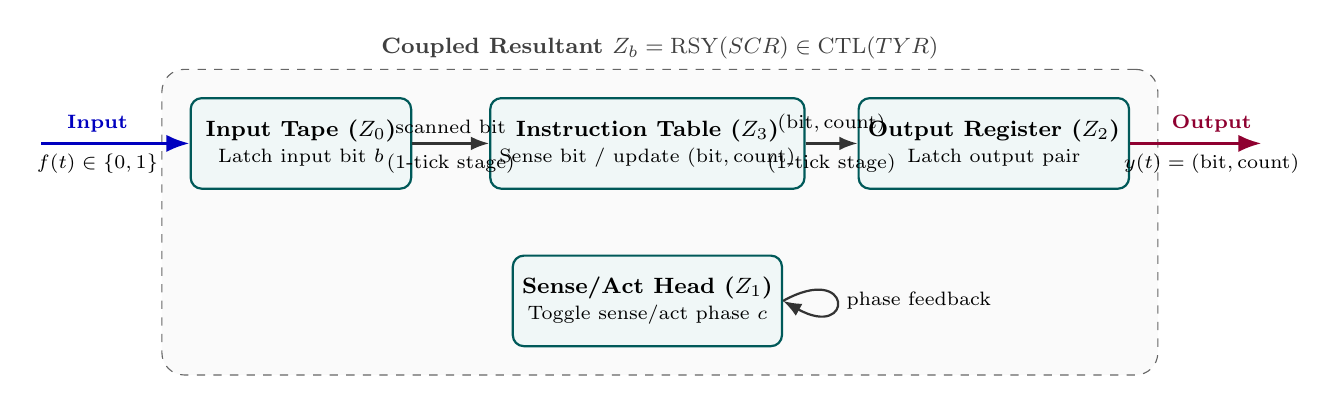
\begin{tikzpicture}[auto, >=Latex, thick,
    comp/.style={draw=teal!70!black, fill=teal!6, rectangle, rounded corners=4pt, minimum width=2.8cm, minimum height=1.15cm, align=center, font=\footnotesize},
    boundary/.style={draw=black!60, dashed, rounded corners=8pt, inner sep=10pt},
    wire/.style={->, >=Latex, thick, draw=black!80},
    port/.style={circle, draw=black!75, fill=white, inner sep=1.6pt}
  ]
    % Components
    \node (tape) [comp] at (0, 1.3) {\textbf{Input Tape ($Z_0$)}\\{\scriptsize Latch input bit $b$}};
    \node (table) [comp] at (4.4, 1.3) {\textbf{Instruction Table ($Z_3$)}\\{\scriptsize Sense bit / update $(\text{bit},\text{count})$}};
    \node (reg) [comp] at (8.8, 1.3) {\textbf{Output Register ($Z_2$)}\\{\scriptsize Latch output pair}};
    \node (head) [comp] at (4.4, -0.7) {\textbf{Sense/Act Head ($Z_1$)}\\{\scriptsize Toggle sense/act phase $c$}};

    % System boundary box
    \begin{scope}[on background layer]
      \node (sysbox) [boundary, fill=gray!4, fit=(tape)(table)(reg)(head), label={[font=\footnotesize\bfseries, text=black!75]above:Coupled Resultant $Z_b = \mathrm{RSY}(SCR) \in \mathrm{CTL}(TYR)$}] {};
    \end{scope}

    % External Input
    \draw[wire, draw=blue!75!black, very thick] (-3.3, 1.3) -- node[above, pos=0.38, font=\scriptsize\bfseries, text=blue!75!black] {Input} node[below, pos=0.38, font=\scriptsize] {$f(t)\in\{0,1\}$} (tape.west);

    % Internal connections
    \draw[wire] (tape.east) -- node[above, font=\scriptsize] {scanned bit} node[below, font=\scriptsize] {(1-tick stage)} (table.west);
    \draw[wire] (table.east) -- node[above, font=\scriptsize] {$(\text{bit},\text{count})$} node[below, font=\scriptsize] {(1-tick stage)} (reg.west);

    % Head self-loop
    \draw[wire] (head.east) .. controls +(0.9,0.5) and +(0.9,-0.5) .. node[right, font=\scriptsize] {phase feedback} (head.east);

    % External Output
    \draw[wire, draw=purple!75!black, very thick] (reg.east) -- node[above, pos=0.62, font=\scriptsize\bfseries, text=purple!75!black] {Output} node[below, pos=0.62, font=\scriptsize] {$y(t)=(\text{bit},\text{count})$} (12.2, 1.3);
  \end{tikzpicture}%
  }
  \caption{System coupling recipe $SCR$ for the four-component streaming Run-Length Encoder. Because resultants update synchronously from pre-step readouts, the internal connections from Input Tape ($Z_0$) to Instruction Table ($Z_3$) and from Instruction Table ($Z_3$) to Output Register ($Z_2$) form a two-stage Moore pipeline.}
  \label{fig:rle-architecture}
\end{figure*}

As shown in Figure~\ref{fig:rle-architecture}, the coupling recipe $SCR$ connects the tape's output port to the instruction table's input port, connects the instruction table's output port to the output register's input port, and closes the head's auxiliary port with a self-loop. This leaves a single unconnected system input $\mathrm{UISCR}(SCR)$ (the external bit stream $f(t)$ arriving at the tape) and a single unconnected system output $\mathrm{UOSCR}(SCR)$ (the encoded pair $y(t)=(\text{bit},\text{count})$ emitted by the output register).

\subsubsection{Stage 1: Idealized Infinite-Tape Specification (\texorpdfstring{$IOR_\infty$}{IOR\_inf})}
\label{sec:case-machine-reference}
In the initial specification stage, we define the idealized mathematical behavior on an unbounded stream of binary inputs $f:\mathbb{N}\to\{0,1\}$ with no upper bound on run length ($\mathrm{count}\in\mathbb{N}$). One input symbol is sampled per two-tick sense/act cycle, so the $k$-th sampled symbol is $f(2k)$. Comparing consecutive sampled symbols defines the recurrence:
\begin{equation}
\begin{aligned}
  \mathrm{runLen}_\infty(f,0) &= 1, \\
  \mathrm{runLen}_\infty(f,k{+}1) &=
  \begin{cases}
    \mathrm{runLen}_\infty(f,k)+1, & f\bigl(2(k{+}1)\bigr)=f(2k),\\
    1, & \text{otherwise.}
  \end{cases}
\end{aligned}
  \label{eq:rle-inf-recurrence}
\end{equation}
At the instruction table level, the unshifted trajectory $\phi_{\mathrm{out},\infty}(f,t)$ starts at $(0,0)$ for $t=0$, emits $\bigl(f(2k),\mathrm{runLen}_\infty(f,k)\bigr)$ on act completion tick $2k+1$, and holds that pair on sense tick $2k+2$.

In the coupled resultant $\mathrm{RSY}(SCR)$, synchronous Moore communication across the two internal connections (from input tape to instruction table and from instruction table to output register) introduces a two-stage Moore pipeline. Relative to the table-level trajectory $\phi_{\mathrm{out},\infty}$, this shifts the external register output by two ticks ($y(t)=\phi_{\mathrm{out},\infty}(f,t-2)$ for $t\ge 2$). End-to-end, a sampled input $f(2k)$ reaches the boundary register only at tick $2k+3$ (three ticks), because $\phi_{\mathrm{out},\infty}$ already accounts for one table-update tick. Incorporating the two-tick shift of $\phi_{\mathrm{out},\infty}$ into the boundary requirement yields the trajectory predicate $A_{IOR_\infty}(f,y)$ of the idealized boundary specification $\Phi_{IOR_\infty}$:
\begin{equation}
  A_{IOR_\infty}(f,y)
  \;\Longleftrightarrow\;
  G\left(
  y(t)=
  \begin{cases}
    (0,0), & t<2,\\
    \phi_{\mathrm{out},\infty}(f,t-2), & t\ge 2.
  \end{cases}
  \right)
  \label{eq:phi-ior-inf}
\end{equation}
Because $\phi_{\mathrm{out},\infty}(f,0)=(0,0)$, the case $t\ge 2$ also forces $y(2)=(0,0)$, so the register emits the idle pair $(0,0)$ throughout the three-tick startup window $t=0,1,2$. For example, when input symbols $0,0,1$ arrive at ticks $0,2,4$, the output register emits $(0,0)$ during those startup ticks and then emits $(0,1)$, $(0,2)$, and $(1,1)$ at ticks $3,5,7$ (holding each pair across the subsequent even tick). While $IOR_\infty$ and its unbounded resultant $Z_{b,\infty}$ provide a relatively clean mathematical baseline, their state spaces are countably infinite ($\mathrm{count}\in\mathbb{N}$) and therefore cannot be realized in finite digital hardware or exhaustively checked by a finite-state model checker.  %We could find, however, a proof by other means, e.g., inductive invariants or interactive theorem provers can verify $IOR_\infty$ over unbounded integers, whereas automated finite-state model checking requires bounded operational regimes.

\subsubsection{Stage 2: Buildable Finite-Tape Machine (\texorpdfstring{$Z_{b,N}$ and $Z_{m,N}$}{Zb,N and Zm,N})}
\label{sec:case-machine-zones}
To move from the idealized specification to a physically buildable machine, we refine the technology catalog to $TYR_N$, where the counter register in each component has a finite hardware capacity $N\ge 1$ ($\mathrm{count}\in\{0,1,\dots,N\}$). Correspondingly, the refined boundary requirement $IOR_N$ caps consecutive run counts at saturating capacity $N$:
\begin{equation}
\begin{aligned}
  \mathrm{runLen}_N(f,0) &= \min(1,N), \\
  \mathrm{runLen}_N(f,k{+}1) &=
  \begin{cases}
    \min(\mathrm{runLen}_N(f,k){+}1,N),\\
    \hspace{2.5em}\text{if } f(2k{+}2)=f(2k),\\
    \min(1,N),\quad \text{otherwise.}
  \end{cases}
\end{aligned}
  \label{eq:rle-fin-recurrence}
\end{equation}
For every input run of length at most $N$, the finite-tape trajectory $\phi_{\mathrm{out},N}(f,t)$ is identical to the unbounded trajectory $\phi_{\mathrm{out},\infty}(f,t)$, while runs exceeding $N$ saturate at $N$.

Because every component $Z_{0,N},Z_{1,N},Z_{2,N},Z_{3,N}\in TYR_N$ is a finite discrete system, the coupled resultant $Z_{b,N}=\mathrm{RSY}(SCR_N)\in\mathrm{CTL}(TYR_N)$ is a finite-state machine. Furthermore, when initialized in its all-zero reset configuration $s_{b,0}$, the resultant's reachable operational behavior forms a finite system mode $Z_{m,N}\in\mathrm{SYSMO}(Z_{b,N})$ whose state space $S_{m,N}$ is a fraction of the full Cartesian product $\prod_{i=0}^3 S_{i,N}$ (for example, at capacity $N=3$, the full resultant has $512$ states whereas the active system mode $Z_{m,3}$ has $43$ reachable states).

By Theorem~\ref{thm:mode-ior-bridge} and Theorem~\ref{thm:dynamics-characterization}, we can certify that $(D_{\mathrm{ref},N},Z_{b,N})$ belongs to the implementability cotyledon $\mathrm{CTL}(IOR_N,TYR_N)$ either by checking $Z_{m,N}\models_{IO}\Phi_{IOR_N}$ directly on the boundary ports or by checking $Z_{m,N}\models_{\mathrm{dyn}}\Phi_{\mathrm{dyn}}(Z_{\mathrm{ref},N})$ against the pipeline reference design $Z_{\mathrm{ref},N}\in\mathrm{CTL}(IOR_N)$.

\subsection{Automated LTL Verification of Buildable System Modes}
\label{sec:case-solver}

Once the finite-capacity technology catalog $TYR_N$ is fixed, the boundary specification $\Phi_{IOR_N}$ of Equation~\eqref{eq:rle-fin-recurrence} compiles into six families of propositional LTL clauses. Writing $f\in\{0,1\}$ for the boundary input bit $f(t)$, $y=(y_{\mathrm{bit}},y_{\mathrm{cnt}})\in\{0,1\}\times\{0,\dots,N\}$ for the boundary register output pair $y(t)$ (using $y=(b,k)$ as shorthand for $y_{\mathrm{bit}}=b \wedge y_{\mathrm{cnt}}=k$), and $c\in\{0,1\}$ for the sense/act head phase $c(t)$, Table~\ref{tab:rle-ltl-clauses} summarizes the compiled clause families comprising $\Phi_{IOR_N}$ along with their count and derivation from the boundary recurrence~\eqref{eq:rle-fin-recurrence}. Here $X^k$ denotes $k$ consecutive next-step operators ($X^3 \equiv XXX$), reflecting the three-tick end-to-end pipeline latency. Together, these six families contribute $1+1+2N+2+2N+2N = 6N+4$ propositional LTL clauses at capacity $N$.

\begin{table*}[t]
\caption{Propositional LTL compilation of the finite-tape boundary specification $\Phi_{IOR_N}$ from recurrence~\eqref{eq:rle-fin-recurrence}.}
\label{tab:rle-ltl-clauses}
\renewcommand{\arraystretch}{1.25}
\footnotesize
\begin{tabularx}{\textwidth}{@{}l >{$}l<{$} c X@{}}
\toprule
\textbf{Clause} & \textbf{Propositional LTL Formula} & \textbf{Count} & \textbf{Derivation from Boundary Requirement $IOR_N$} \\
\midrule
$\varphi_{\mathrm{init}}$ & (y{=}(0,0)) \wedge X(y{=}(0,0)) \wedge X^2(y{=}(0,0)) & 1 & Forces the idle pair $(0,0)$ across the three-tick pipeline startup window ($t=0,1,2$) before the first encoded symbol emerges. \\
$\varphi_{\mathrm{mode}}$ & G\bigl((c{=}0 \leftrightarrow X(c{=}1)) \wedge (c{=}1 \leftrightarrow X(c{=}0))\bigr) & 1 & Enforces the two-phase alternating clock discipline (sense: $c=0$, act: $c=1$) governing the synchronous Moore pipeline. \\
$\varphi_{\mathrm{hold}}$ & G\bigl((c{=}1 \wedge y{=}(b,k)) \rightarrow X(y{=}(b,k))\bigr),\ b\in\{0,1\}, k\in\{1,\dots,N\} & 2N & Requires the output register to hold a valid run pair $(b,k)$ across the second half of each two-phase cycle, matching the step-synchronous spec. \\
$\varphi_{\mathrm{start}}$ & G\bigl((c{=}0 \wedge f{=}b \wedge X(y_{\mathrm{cnt}}{=}0)) \rightarrow X^3(y{=}(b,1))\bigr),\ b\in\{0,1\} & 2 & Translates the base case $\ell_N(f,0)=1$ of~\eqref{eq:rle-fin-recurrence}, emitting the initial run pair $(b,1)$ after the three-tick pipeline latency ($X^3$). \\
$\varphi_{\mathrm{inc}}$ & G\bigl((c{=}0 \wedge f{=}b \wedge X(y{=}(b,k))) \rightarrow X^3(y{=}(b,\min(k{+}1,N)))\bigr),\ k\le N & 2N & Translates the matching-symbol recurrence ($\ell_N(f,k{+}1)=\min(\ell_N(f,k){+}1,N)$ for $f(2k{+}2)=f(2k)$), incrementing the count with capacity saturation. \\
$\varphi_{\mathrm{reset}}$ & G\bigl((c{=}0 \wedge f{=}b \wedge X(y{=}(\neg b,k))) \rightarrow X^3(y{=}(b,1))\bigr),\ k\le N & 2N & Translates the run-breaking recurrence ($\ell_N(f,k{+}1)=1$ for $f(2k{+}2)\neq f(2k)$), resetting the counter to $1$ and updating the active symbol bit. \\
\midrule
\multicolumn{2}{@{}l}{\textbf{Total Propositional Clauses ($N$-capacity):}} & \textbf{6N+4} & 16 ($N{=}2$), 22 ($N{=}3$), 28 ($N{=}4$) across all six families. \\
\bottomrule
\end{tabularx}
\end{table*}

We implemented an automated verification workflow in Python (3.12) on Ubuntu 24.04 under Windows Subsystem for Linux 2 (WSL2). Given a candidate component catalog $TYR_N$ and coupling recipe $SCR_N$, the workflow constructs the coupled resultant $Z_{b,N}=\mathrm{RSY}(SCR_N)$, isolates the reachable operational system mode $Z_{m,N}\in\mathrm{SYSMO}(Z_{b,N})$ from the initial reset state, and checks the boundary LTL specification $\Phi_{IOR_N}$ (Table~\ref{tab:rle-ltl-clauses}) by explicit-state exploration of that mode. Table~\ref{tab:solver-results} reports those $\Phi_{IOR_N}$ proof-of-concept results. When a prescribed reference $Z_{\mathrm{ref},N}$ is in view, Theorem~\ref{thm:dynamics-characterization} still applies: $Z_{m,N}\models_{\mathrm{dyn}}\Phi_{\mathrm{dyn}}(Z_{\mathrm{ref},N})$ is the existential SAT query $\exists(h_S,h_I,h_O)$ (functionality, readout/step preservation, and surjectivity), which can be discharged by a propositional encoding in Z3~\cite{deMouraZ32008} that discovers the maps rather than requiring a hand-written architectural projection. In the nominal four-component architecture, the input tape ($|S_0|=2$), sense/act head ($|S_1|=2$), output register ($|S_2|=2(N{+}1)$), and instruction table ($|S_3|=4(N{+}1)$) form a Cartesian product resultant state space of size $|S_{\mathrm{resultant}}|=32(N{+}1)^2$, whereas synchronous coupling restricts the reachable operational mode $Z_{m,N}$ to a much smaller invariant sub-system $|S_{\mathrm{mode}}|$.

\begin{table*}[t]
\caption{Automated boundary LTL verification results for finite-tape buildable RLE resultants $Z_{b,N}=\mathrm{RSY}(SCR_N)$ and their operational system modes $Z_{m,N}\in\mathrm{SYSMO}(Z_{b,N})$ against $\Phi_{IOR_N}$.}
\label{tab:solver-results}
\renewcommand{\arraystretch}{1.25}
\footnotesize
\begin{tabularx}{\textwidth}{@{}X r r r r c c r@{}}
\toprule
\textbf{Candidate Design} & \textbf{Cap $N$} & \textbf{$|S_{\mathrm{resultant}}|$} & \textbf{$|S_{\mathrm{mode}}|$} & \textbf{Clauses} & \textbf{Verdict} & \textbf{Violated} & \textbf{Wall time (ms)} \\
\midrule
\csname @@input\endcsname generated/solver-results.tex
\bottomrule
\end{tabularx}
\end{table*}

The nine candidate designs in Table~\ref{tab:solver-results} are organized into three evaluation groups that test capacity scaling, subsystem refactoring invariance, and fault and timing-mismatch diagnosis.

The first three rows (\emph{Baseline coupled RLE} for $N=2,3,4$) evaluate how verification scales as the hardware counter capacity $N$ of the technology catalog $TYR_N$ increases. Each design is constructed by interconnecting the nominal input tape ($Z_0$), sense/act head ($Z_1$), output register ($Z_2$), and instruction table ($Z_3$) through the coupling recipe $SCR_N$ of Figure~\ref{fig:rle-architecture}, with the count registers in $Z_2$ and $Z_3$ bounded to $\{0,\dots,N\}$. Increasing $N$ from $2$ to $4$ expands the coupled resultant state space $|S_{\mathrm{resultant}}|$ from $288$ to $800$ states and the reachable operational mode $|S_{\mathrm{mode}}|$ from $31$ to $55$ states ($12N+7$). All three designs pass all $6N+4$ LTL clauses ($16$, $22$, and $28$ clauses, respectively). By Theorem~\ref{thm:mode-ior-bridge}, each PASS verdict on $\Phi_{IOR_N}$ certifies that $(D_{m,N},Z_{b,N})\in\mathrm{CTL}(IOR_N,TYR_N)$ for the mode-as-functional-design $D_{m,N}=(Z_{m,N},s_{b,0},T)$, without requiring manual construction of a state-space map $h_S$.

The next two rows (\emph{Phase-inverted instruction table} and \emph{Parity-instrumented output register}, both at $N=3$) test whether boundary and dynamics-fragment verification remain invariant when subsystem teams refactor internal state representations or elaborate components with auxiliary diagnostic state. Both candidates modify a single component within the nominal $N=3$ coupling recipe $SCR_3$. The \emph{phase-inverted instruction table} design replaces $Z_3$ with an isomorphic component $Z_3'$ whose internal sense/act phase bit is inverted ($0\leftrightarrow 1$) together with its transition and readout tables, leaving $|S_{\mathrm{resultant}}|=512$ and $|S_{\mathrm{mode}}|=43$ unchanged. The \emph{parity-instrumented output register} design replaces $Z_2$ with an elaborated register $Z_2^+$ whose state space $S_2\times\{0,1\}$ appends an internal diagnostic parity bit that toggles on each processed input bit while emitting the same boundary pair $(\text{bit},\text{count})$; this doubles the resultant state space from $512$ to $1024$ states and expands the reachable operational mode from $43$ to $79$ states. Both designs pass all clauses of $\Phi_{IOR_3}$ without any change to the requirement specification. Whereas classical T3SD verification would in general require rewriting an explicit state homomorphism $h_S$ to decode the inverted phase bit in $Z_3'$ or project away the diagnostic parity state in $Z_2^+$, Theorems~\ref{thm:encoding-invariance} and~\ref{thm:elaboration-coupling} ensure that boundary temporal satisfaction absorbs internal re-encodings and state elaborations automatically, certifying that both refactored architectures remain in $\mathrm{CTL}(IOR_3,TYR_3)$.

The final four rows evaluate diagnostic rejection when a component in $TYR_3$ violates its behavioral contract or when the specification clock is misaligned with the hardware pipeline. The \emph{stuck sense/act head} design replaces $Z_1$ with a faulty head whose transition map fails to toggle and remains fixed in its initial phase; the checker rejects the resultant on the phase-alternation clause $\varphi_{\mathrm{mode}}$. The \emph{frozen input tape} design replaces $Z_0$ with a faulty tape whose transition map ignores incoming external bits and permanently retains its initial $0$ bit; because a $1$ bit is never latched, the reachable operational mode collapses from $43$ states to $9$ states and the checker rejects the design on the initial symbol-acquisition clause $\varphi_{\mathrm{start}}$. The \emph{non-resetting instruction table} design replaces $Z_3$ with a faulty table that continues incrementing the run count (up to $N=3$) when the input bit changes instead of resetting the count to $1$; although the resultant reaches $43$ mode states and satisfies the startup, hold, and same-bit increment clauses, the checker rejects it on the run-reset clause $\varphi_{\mathrm{reset}}$. Finally, the \emph{unshifted single-tick specification} candidate pairs the nominal, fault-free $N=3$ coupled resultant ($|S_{\mathrm{resultant}}|=512$, $|S_{\mathrm{mode}}|=43$) against an idealized single-tick requirement that expects the boundary output to update on every clock tick rather than holding across the two-phase sense/act cycle. The checker rejects this pairing on $\varphi_{\mathrm{hold}}$, confirming empirically the timing-alignment requirement discussed in Section~\ref{sec:case-machine}: even when the underlying hardware components are sound, no lock-step Wymore homomorphism exists unless the specification and the buildable resultant share a matched clock granularity.


\section{Discussion} \label{sec:discussion}

\subsection{Why Temporal Logic Unlocks Scalable T3SD Verification}
\label{sec:implications}

Wymore's Tricotyledon Theory of System Design offers one of the most mathematically rigorous foundations in systems engineering: it cleanly separates what a system must do at its boundary ($\mathrm{CTL}(IOR)$) from how a system is built out of available components ($\mathrm{CTL}(TYR)$), and defines implementability ($\mathrm{CTL}(IOR,TYR)$) via homomorphisms from operational system modes $Z_m\in\mathrm{SYSMO}(Z_b)$ onto functional designs $Z_f\in\mathrm{CTL}(IOR)$. Yet despite its conceptual clarity, T3SD never achieved widespread industrial adoption for formal verification. A primary reason is sociological and tool-related: the T3SD community remained relatively small and never developed automated solver ecosystems comparable to those built over four decades by the formal methods and model-checking communities \citep{Pnueli1977,MannaPnueli1995,BiereCimattiClarkeZhu1999,BaierKatoen2008}. Consequently, applying T3SD required constructing and maintaining explicit state-space homomorphisms $h=(h_S,h_I,h_O)$ by hand---an approach that quickly becomes intractable as coupled architectures grow in state count and undergo iterative design revisions.

The bridge established in this paper shows that systems engineers do not need to choose between Wymore's architectural rigor and modern automated verification:
\begin{itemize}
    \item \textbf{Isomorphic requirement representation ($\Phi_{IOR}$):} Theorem~\ref{thm:boundary-characteristic} proves that Wymore's $IOR$ is canonically isomorphic to a boundary temporal specification $\Phi_{IOR}$. Expressing $ER(f)$ in temporal logic loses none of T3SD's trajectory semantics while making causality constraints---such as why $\mathrm{CTL}(IOR_{\mathrm{echo}})=\emptyset$ and why multi-stage pipeline latency must appear in $\Phi_{IOR_{\mathrm{RLE}}}$---immediately visible.
    \item \textbf{Eliminating manual homomorphism search on finite buildable modes:} While idealized mathematical specifications ($IOR_\infty$) may involve infinite state spaces, every physical or digital component in a real-world technology catalog $TYR$ is finite. Thus every buildable resultant $Z_b=\mathrm{RSY}(SCR)\in\mathrm{CTL}(TYR)$ and every operational mode $Z_m\in\mathrm{SYSMO}(Z_b)$ is a finite Kripke structure. By Theorem~\ref{thm:mode-ior-bridge} and Theorem~\ref{thm:dynamics-characterization}, checking whether $Z_b$ belongs to the implementability cotyledon $\mathrm{CTL}(IOR,TYR)$ reduces to decidable LTL model checking ($Z_m\models_{IO}\Phi_{IOR}$ or $Z_m\models_{\mathrm{dyn}}\Phi_{\mathrm{dyn}}(Z_{\mathrm{ref}})$).
    \item \textbf{Resilience to architectural refactoring:} As demonstrated in Table~\ref{tab:solver-results} (\texttt{rle-reencoded-table} and \texttt{rle-instrumented-reg}), when a subsystem team re-encodes a component's internal state or elaborates a component with diagnostic instrumentation, the temporal specifications $\Phi_{IOR}$ and $\Phi_{\mathrm{dyn}}$ remain completely unchanged. The model checker automatically re-verifies the modified mode without requiring a human engineer to reconstruct the state projection $h_S$.
\end{itemize}

\subsection{Complementary Roles of \texorpdfstring{$\Phi_{IOR}$ and $\Phi_{\mathrm{dyn}}$}{Phi\_IOR and Phi\_dyn}}
\label{sec:limitations}

Our framework provides two distinct temporal verification targets corresponding to two stages of the systems engineering lifecycle:
\begin{enumerate}
    \item \textbf{Direct boundary verification ($Z_m\models_{IO}\Phi_{IOR}$):} When the engineering requirement is specified purely in terms of input/output trajectories (such as Equations~\eqref{eq:ltl-init}--\eqref{eq:ltl-reset} for the finite-tape RLE), Theorem~\ref{thm:mode-ior-bridge} certifies membership in $\mathrm{CTL}(IOR,TYR)$ directly from the boundary behavior of the mode $Z_m$, without requiring the engineer to first design an intermediate reference state machine $Z_{\mathrm{ref}}$.
    \item \textbf{Reference-dynamics verification ($Z_m\models_{\mathrm{dyn}}\Phi_{\mathrm{dyn}}(Z_{\mathrm{ref}})$):} When a reference functional architecture $D_{\mathrm{ref}}=(Z_{\mathrm{ref}},s_0,T)\in\mathrm{CTL}(IOR)$ has already been established as a golden specification and subsystem teams are elaborating its components, Theorem~\ref{thm:dynamics-characterization} and Theorem~\ref{thm:elaboration-coupling} verify that the detailed mode $Z_m$ is a true homomorphic elaboration of $Z_{\mathrm{ref}}$.
\end{enumerate}
Separating these two checks also sharpens failure diagnosis. If a candidate mode $Z_m$ fails $\Phi_{IOR}$, it violates the stakeholder boundary requirement outright and cannot belong to $\mathrm{CTL}(IOR)$. If $Z_m$ satisfies $\Phi_{IOR}$ on the boundary but fails $\Phi_{\mathrm{dyn}}(Z_{\mathrm{ref}})$, then $Z_m$ is a valid functional realization of $IOR$ that achieves the required behavior through a different internal state organization or timing decomposition than the chosen reference machine $Z_{\mathrm{ref}}$.

\subsection{Scope, Clock Granularity, and Future Directions}
\label{sec:future}

Several extensions follow naturally from the results established here:
\begin{itemize}
    \item \textbf{Multi-rate and stuttering implementation relations:} Because a classical Wymore homomorphism is a lock-step map ($1$ mode tick $= 1$ reference tick), staged implementations with multi-tick sense/act cycles or pipeline stages must match the clock granularity of the reference specification (Proposition~\ref{prop:matched-ticks}). Relaxing lock-step homomorphisms to $k$-tick or stuttering bisimulation relations---translated into LTL without the next-step operator $X$ \citep{Lamport2002,BrowneClarkeGrumberg1988}---would allow multi-rate modes to be verified against unpipelined abstract references.
    \item \textbf{Companion liveness and fairness specifications:} The dynamics fragment $\Phi_{\mathrm{dyn}}$ uses only safety operators ($G$ and $X$) because Wymore's homomorphism equations~\eqref{eq:wymore-hom-def} are step-local invariants. Richer temporal liveness requirements---such as eventual buffer drainage ($GF\,\mathit{empty}$) or starvation-free arbitration---can be included directly in $\Phi_{IOR}$ and checked alongside $\Phi_{\mathrm{dyn}}$ by the same LTL model-checking engine.
    \item \textbf{Symbolic BDD and SAT-based model checking at industrial scale:} While explicit-state reachability and LTL checking in \texttt{scripts/ltl\_ior\_checker.py} discharge our coupled RLE modes in milliseconds, larger industrial couplings with $10^6$ or more reachable mode states can leverage symbolic model checkers (such as {NuSMV}/{nuXmv}~\citep{CavadaEtAl2014}) and compositional lifting (Theorem~\ref{thm:elaboration-coupling}) to verify each component in $TYR$ locally before lifting conformance to $\mathrm{RSY}(SCR)$.
\end{itemize}

\section{Conclusions}
\label{sec:conclusions}

This paper has shown that Wymore's Tricotyledon Theory of System Design (T3SD) can be connected directly to the methods and automated verification tools of temporal logic without altering T3SD's mathematical foundations. Specifically:
\begin{enumerate}
    \item Every Wymorian Input/Output Requirement $IOR$ translates into an isomorphic boundary temporal specification $\Phi_{IOR}$ whose assertional satisfaction space $\mathrm{AFSR}(\Phi_{IOR})$ is in canonical bijection with the functionality cotyledon $\mathrm{CTL}(IOR)=\mathrm{FSR}(IOR)$ (Theorem~\ref{thm:boundary-characteristic}).
    \item Selecting an operational system mode $Z_m\in\mathrm{SYSMO}(Z_b)$ of a buildable resultant $Z_b=\mathrm{RSY}(SCR)\in\mathrm{CTL}(TYR)$, boundary temporal satisfaction $Z_m\models_{IO}\Phi_{IOR}$ is necessary and sufficient for the existence of an identity-boundary homomorphism onto a functional design in $\mathrm{CTL}(IOR)$, certifying membership in the implementability cotyledon $\mathrm{CTL}(IOR,TYR)$ without manual homomorphism construction (Theorem~\ref{thm:mode-ior-bridge}).
    \item Compiling a chosen reference functional design $Z_{\mathrm{ref}}\in\mathrm{CTL}(IOR)$ into the step-local safety fragment $\Phi_{\mathrm{dyn}}(Z_{\mathrm{ref}})$ makes assertional satisfaction $Z_m\models_{\mathrm{dyn}}\Phi_{\mathrm{dyn}}(Z_{\mathrm{ref}})$ logically equivalent to the existence of a surjective Wymore homomorphism $h:Z_m\twoheadrightarrow Z_{\mathrm{ref}}$, while remaining invariant under isomorphic state re-encodings, port copies, and compositional coupling (Theorems~\ref{thm:dynamics-characterization}--\ref{thm:finite-canonicity}).
    \item Because physically buildable components in $TYR$ are finite-state, refining an idealized infinite-tape streaming Run-Length Encoder ($IOR_\infty$) to a finite-tape buildable resultant $Z_{b,N}=\mathrm{RSY}(SCR_N)$ allows an automated LTL checker to verify active system modes $Z_{m,N}\in\mathrm{SYSMO}(Z_{b,N})$, tolerate internal component refactorings with zero specification maintenance, and diagnose component faults and pipeline timing mismatches in milliseconds.
\end{enumerate}
By importing decidable temporal logic verification into T3SD, systems engineers can verify significantly larger and more complex coupled architectures inside Wymore's tricotyledon framework than was previously practical by hand.


\bibliographystyle{ama}
\bibliography{refs}

% ----- Appendices -----
\appendix
% \appendix

% \section{Pathological Buildability Without Implementability}
% \label{app:pathology}

% This appendix tries to answer the questions raised by Figure~\ref{fig:t3sd-cotyledons}: can a buildable system $Z_{\text{impl}}$ satisfy a property set $\Phi$ while lying outside the implementability cotyledon? That is, with no Wymore homomorphism to a reference system that expresses the same functional intent. We give a few sketches, but neither is a finished theorem in this paper.  Both are meant to explore the question.

% \subsection{What Would Count as Pathology?}

% Recall that classical implementability requires a homomorphism $h = (h_S, h_I, h_O)$ from $Z_{\text{impl}}$ to $Z_{\text{spec}}$ with surjective component maps and tick-wise preservation:
% \begin{align}
%     h_S(\delta_{\text{impl}}(s, i)) &= \delta_{\text{spec}}(h_S(s), h_I(i)), \label{eq:delta-preserve}\\
%     h_O(\rho_{\text{impl}}(s)) &= \rho_{\text{spec}}(h_S(s)). \label{eq:rho-preserve}
% \end{align}
% Assertional membership requires only $Z_{\text{impl}} \models_{\mathcal{L}} \Phi$ over admissible boundary trajectories.

% A \emph{pathological witness} (for our purposes) is a triple $(Z_{\text{impl}}, \Phi, \mathcal{Z})$ where:
% \begin{enumerate}
%     \item $Z_{\text{impl}}$ is buildable (technology-feasible in the BC sense used in the main text);
%     \item $Z_{\text{impl}} \models_{\mathcal{L}} \Phi$;
%     \item $\mathcal{Z}$ is a class of reference systems intended to represent the same functional intent as $\Phi$; and
%     \item there is no $Z_{\text{spec}} \in \mathcal{Z}$ and no homomorphism $h : Z_{\text{impl}} \to Z_{\text{spec}}$ satisfying \eqref{eq:delta-preserve}--\eqref{eq:rho-preserve}.
% \end{enumerate}
% The subtlety is item~(3). Classical T3SD does not designate a \emph{unique} $Z_{\text{spec}}$ for a requirement; engineers may choose among reference designs. A pathology that disappears as soon as one picks a different $Z_{\text{spec}}$ tailored to the implementation is weaker than one that persists against a natural family of references.

% If ``equivalent specification'' means ``some $Z_{\text{spec}}$ for which an $h$ exists,'' then the question collapses: one could always try to build $Z_{\text{spec}}$ as a homomorphic image of $Z_{\text{impl}}$ via Wymore's HIMSY construction \parencite{Wymore1993}. That image simulates the implementation by construction but may be \emph{more detailed} than the conceptual requirement and may not be the reference a systems engineer wanted. The interesting gap is between stakeholder-level $\Phi$ (or a compact conceptual $Z_{\text{spec}}$) and buildable $Z_{\text{impl}}$, not between $Z_{\text{impl}}$ and its own collapsed image.

% \subsection{Example 1: Deterministic Resolution of Disjunctive Intent}
% \label{app:deterministic-resolution}

% \paragraph{Property.} A fault-handling requirement with unresolved design choice:
% \[
%     \varphi_{\text{fault}} \;=\; G\bigl(\mathit{fault} \rightarrow X(\mathit{engine\_A} \lor \mathit{engine\_B})\bigr).
% \]
% The stakeholder allows either backup engine; the implementation team commits to~A.

% \paragraph{Reference system $Z_{\text{spec}}$ (naive constructive encoding).} Because Wymore systems are deterministic, a single $Z_{\text{spec}}$ that genuinely branches on ``A or B'' without committing must encode the choice in inputs. A standard construction enlarges the input space:
% \begin{center}
% \small
% \begin{tabular}{@{}ll@{}}
%     $I_{\text{spec}}$ & $\{\mathit{nominal}, \mathit{fault}\} \times \{\mathit{envA}, \mathit{envB}\}$ \\
%     $S_{\text{spec}}$ & $\{s_0, s_A, s_B\}$ \\
%     $\delta_{\text{spec}}$ & $s_0 \xrightarrow{(\mathit{fault},\mathit{envA})} s_A$;\quad $s_0 \xrightarrow{(\mathit{fault},\mathit{envB})} s_B$ \\
%     $\rho_{\text{spec}}$ & $\mathit{engine\_A}$ at $s_A$;\quad $\mathit{engine\_B}$ at $s_B$
% \end{tabular}
% \end{center}
% This $Z_{\text{spec}}$ is $\Phi$-adequate in the sense that each admissible resolution is realizable.

% \paragraph{Buildable implementation $Z_{\text{impl}}$.} The physical controller exposes only $\{\mathit{nominal}, \mathit{fault}\}$ and hardwires engine~A:
% \begin{center}
% \small
% \begin{tabular}{@{}ll@{}}
%     $I_{\text{impl}}$ & $\{\mathit{nominal}, \mathit{fault}\}$ \\
%     $S_{\text{impl}}$ & $\{q_0, q_A\}$ \\
%     $\delta_{\text{impl}}$ & $q_0 \xrightarrow{\mathit{fault}} q_A$ \\
%     $\rho_{\text{impl}}$ & $\mathit{engine\_A}$ at $q_A$
% \end{tabular}
% \end{center}

% \paragraph{Assertional success.} On every admissible trace, $\mathit{fault}$ at tick~$t$ yields $\mathit{engine\_A}$ at $t{+}1$, so $\mathit{engine\_A} \lor \mathit{engine\_B}$ holds. Thus $Z_{\text{impl}} \models \varphi_{\text{fault}}$.

% \paragraph{Homomorphism failure.} Any $h_I : I_{\text{impl}} \twoheadrightarrow I_{\text{spec}}$ requires $|I_{\text{impl}}| \ge |I_{\text{spec}}|$. Here $|I_{\text{impl}}| = 2 < 4 = |I_{\text{spec}}|$, so surjective $h_I$ is impossible and $Z_{\text{impl}}$ cannot lie in IC relative to this $Z_{\text{spec}}$.

% \paragraph{But not quite...} A T3SD-head has two immediate replies:
% \begin{itemize}
%     \item \textbf{Multiple reference systems.} Replace the single branching $Z_{\text{spec}}$ with two references $Z_{\text{spec}}^{(A)}$ and $Z_{\text{spec}}^{(B)}$, one per resolution. Then $Z_{\text{impl}}$ homomorphically maps to $Z_{\text{spec}}^{(A)}$. Functional intent becomes a \emph{set} of specifications, not one 5-tuple.
%     \item \textbf{Wrong reference.} The naive $Z_{\text{spec}}$ models non-deterministic \emph{intent} by fictitious environment inputs the plant does not possess. One could argue the FC artifact should have been $Z_{\text{spec}}^{(A)}$ all along once engineering commits to~A.
% \end{itemize}
% Example~A therefore shows a workflow mismatch (property-level disjunction vs.\ input-lifted deterministic spec) and a clean cardinality obstruction to $h_I$, but not---by itself---an inescapable separation between $\mathcal{FC}_{\mathcal{L}}(\Phi)$ and IC. It is still useful pedagogy: assertional checking accepts the committed implementation without forcing engineers to maintain a four-port fictional environment.

% \subsection{Example 2: Temporal Granularity (Stuttering Internals)}
% \label{app:stuttering}

% Example~B targets tick-for-tick preservation \eqref{eq:delta-preserve} when $\Phi$ uses eventualities that ignore internal timing.

% \paragraph{Property.}
% \[
%     \varphi_{\text{brake}} \;=\; G\bigl(\mathit{obstacle} \rightarrow F\,\mathit{brake\_on}\bigr),
% \]
% interpreted over output readouts at tick boundaries.

% \paragraph{Conceptual reference $Z_{\text{spec}}$.} A minimal two-state intent machine:
% \begin{center}
% \small
% \begin{tabular}{@{}ll@{}}
%     $I_{\text{spec}}$ & $\{\mathit{none}, \mathit{obstacle}\}$ \\
%     $S_{\text{spec}}$ & $\{\mathit{Clear}, \mathit{Braking}\}$ \\
%     $\delta_{\text{spec}}$ & $\mathit{Clear} \xrightarrow{\mathit{obstacle}} \mathit{Braking}$;\; $\mathit{Braking}$ self-loops on $\mathit{none}$ \\
%     $\rho_{\text{spec}}$ & $\mathit{brake\_off}$ at $\mathit{Clear}$;\; $\mathit{brake\_on}$ at $\mathit{Braking}$
% \end{tabular}
% \end{center}
% This is the reference a requirements engineer might draw on a whiteboard: obstacle in one tick, brakes engaged ``immediately'' at the conceptual level.

% \paragraph{Buildable implementation $Z_{\text{impl}}$.} A microprocessor pipeline with three internal ticks before hydraulic pressure reaches the pads; autonomous micro-steps use input $\mathit{none}$ (hold-last-input in the main text's convention):
% \begin{center}
% \small
% \begin{tabular}{@{}ll@{}}
%     $I_{\text{impl}}$ & $\{\mathit{none}, \mathit{obstacle}\}$ \\
%     $S_{\text{impl}}$ & $\{q_{\mathit{clear}}, q_{\mathit{compute}}, q_{\mathit{arm}}, q_{\mathit{brake}}\}$ \\
%     $\delta_{\text{impl}}$ & $q_{\mathit{clear}} \xrightarrow{\mathit{obstacle}} q_{\mathit{compute}} \xrightarrow{\mathit{none}} q_{\mathit{arm}} \xrightarrow{\mathit{none}} q_{\mathit{brake}}$ \\
%     $\rho_{\text{impl}}$ & $\mathit{brake\_off}$ on $\{q_{\mathit{clear}}, q_{\mathit{compute}}, q_{\mathit{arm}}\}$;\; $\mathit{brake\_on}$ on $q_{\mathit{brake}}$
% \end{tabular}
% \end{center}

% \paragraph{Assertional success.} After $\mathit{obstacle}$, readout becomes $\mathit{brake\_on}$ within three ticks, so $F\,\mathit{brake\_on}$ holds on the output trace. Hence $Z_{\text{impl}} \models \varphi_{\text{brake}}$.

% \paragraph{Homomorphism obstruction (sketch).} Suppose $h = (h_S, h_I, h_O)$ satisfies \eqref{eq:delta-preserve}--\eqref{eq:rho-preserve} and $h_I$ is surjective.

% \emph{Step 1 (state image after obstacle).} For $q_{\mathit{clear}}$ and input $\mathit{obstacle}$, \eqref{eq:delta-preserve} gives
% $h_S(q_{\mathit{compute}}) = \delta_{\text{spec}}(h_S(q_{\mathit{clear}}), h_I(\mathit{obstacle}))$.
% The only transition from $\mathit{Clear}$ on $\mathit{obstacle}$ yields $\mathit{Braking}$, so $h_S(q_{\mathit{compute}}) = \mathit{Braking}$.

% \emph{Step 2 (internals must already look ``braking'').} By the same argument applied at $q_{\mathit{compute}}$ and $q_{\mathit{arm}}$ on input $\mathit{none}$, provided $h_I(\mathit{none}) = \mathit{none}$, we obtain $h_S(q_{\mathit{arm}}) = h_S(q_{\mathit{brake}}) = \mathit{Braking}$.

% \emph{Step 3 (readout clash).} Equation~\eqref{eq:rho-preserve} at $q_{\mathit{compute}}$ requires $h_O(\mathit{brake\_off}) = \rho_{\text{spec}}(\mathit{Braking}) = \mathit{brake\_on}$, while at $q_{\mathit{brake}}$ it requires $h_O(\mathit{brake\_on}) = \mathit{brake\_on}$. Thus $h_O$ collapses distinct implementation outputs, and $h_O$ cannot be surjective onto $O_{\text{spec}} = \{\mathit{brake\_off}, \mathit{brake\_on}\}$ unless $|O_{\text{impl}}| = 1$.

% \emph{Alternative branch.} Mapping any internal state to $\mathit{Clear}$ breaks Step~1 at the first $\mathit{none}$-tick: $\delta_{\text{spec}}(\mathit{Clear}, \mathit{none}) = \mathit{Clear}$ but $\delta_{\text{impl}}(q_{\mathit{compute}}, \mathit{none}) = q_{\mathit{arm}}$ maps forward. There is no state in $Z_{\text{spec}}$ that is simultaneously ``conceptually clear'' and ``transiently pre-brake'' under strict $\delta$-preservation.

% \paragraph{But...} Unlike Example~A, proliferating finitely many $Z_{\text{spec}}$ variants (one per pipeline depth) does not obviously patch the gap: any fixed two-state conceptual machine either conflates pre-brake computation with ``braking'' (violating $\rho$) or denies internal progress (violating $\delta$). A family indexed by pipeline depth would be infinite, mirroring the engineering reality that timing refinements are unbounded.

% Remaining caveats:
% \begin{itemize}
%     \item \textbf{Coarser reference.} One could declare $Z_{\text{spec}}$ with a single state and trivial dynamics, homomorphic to everything---but such a reference carries no constructive design content and may not $\Phi$-adequately represent the whiteboard machine above.
%     \item \textbf{HIMSY image.} The homomorphic image of $Z_{\text{impl}}$ is a four-state reference that \emph{does} admit $h$ by construction; again, the gap is between compact intent and buildable detail, not simulability in the abstract.
%     \item \textbf{Formal proof.} A proof of non-existence for a specific witness against a formalized ``$\Phi$-adequate reference'' class remains future work.
% \end{itemize}
  % optional commented sketches
\section{Correspondence Proofs}
\label{app:hom-biimp}

The main text relies on three foundational correspondence results: the boundary isomorphism between $\Phi_{IOR}$ and $\mathrm{CTL}(IOR)$ (Theorem~\ref{thm:boundary-characteristic}), the direct mode-to-$IOR$ implementability equivalence (Theorem~\ref{thm:mode-ior-bridge}), and the dynamics-fragment characterization of Wymore homomorphisms (Theorem~\ref{thm:dynamics-characterization}). We present the self-contained mathematical proofs of these correspondences here.

\subsection{Boundary \texorpdfstring{$IOR$}{IOR}--Temporal Logic Correspondence}

Fix a Wymorian input/output requirement
\[
  IOR=(OLR,IR,ITR,OR,OTR,ER)
\]
and let $T_{IOR}\subseteq\mathbb{N}$ be the operational time scale determined by $OLR$. Its characteristic boundary temporal specification retains the time scale, admissible input trajectories, and eligibility relation:
\[
  \Phi_{IOR}=(T_{IOR},ITR,A_{IOR}),
  \qquad A_{IOR}(f,g)\ \Longleftrightarrow\ g\in ER(f).
\]
For a discrete system $Z=(S,IR,OR,\delta,\rho)$, designated initial state $s_0\in S$, and nonempty operational time scale $T\subseteq T_{IOR}$, the assertional satisfaction condition $Z,s_0,T\models_{IO}\Phi_{IOR}$ requires that for every admissible input $f\in ITR$ and every complete input trajectory $h$ agreeing with $f$ on $T_{IOR}$, the output trajectory $\mathrm{OTZ}(Z,s_0,h)$ generated by $Z$ from $s_0$ agrees on $T$ with some trajectory $g$ satisfying $A_{IOR}(f,g)$.

Substituting the definition $A_{IOR}(f,g)\Longleftrightarrow g\in ER(f)$ transforms ``satisfying $A_{IOR}(f,g)$'' into ``belonging to $ER(f)$.'' Every remaining quantifier and domain condition is identical to Wymore's definition of $\mathrm{SatisfiesIOR}(Z,IOR,s_0,T)$ (Definition~6.31 of \citet{Wymore1993}). Therefore, for every $IOR$ and every tuple $(Z,s_0,T)$,
\[
  Z,s_0,T\models_{IO}\Phi_{IOR}
  \quad\Longleftrightarrow\quad
  \mathrm{SatisfiesIOR}(Z,IOR,s_0,T).
\]
Consequently, a member of $\mathrm{AFSR}(\Phi_{IOR})$ and the corresponding member of $\mathrm{FSR}(IOR)=\mathrm{CTL}(IOR)$ carry the exact same system $Z$, initial state $s_0$, and operational time scale $T$, establishing the canonical bijection $\mathrm{AFSR}(\Phi_{IOR})\simeq\mathrm{FSR}(IOR)=\mathrm{CTL}(IOR)$ of Theorem~\ref{thm:boundary-characteristic}.

To deduce Theorem~\ref{thm:mode-ior-bridge} for a system mode $Z_m=(S_m,IR,OR,\delta_m,\rho_m)\in\mathrm{SYSMO}(Z_b)$ of a buildable resultant $Z_b=\mathrm{RSY}(SCR)\in\mathrm{CTL}(TYR)$:
\begin{itemize}
    \item If $h=(h_S,\mathrm{id}_{IR},\mathrm{id}_{OR}):Z_m\twoheadrightarrow Z_f$ is an identity-boundary homomorphism onto a functional design $D_f=(Z_f,s_{f,0},T)\in\mathrm{CTL}(IOR)$ with $h_S(s_{m,0})=s_{f,0}$, then by induction on $t\in\mathbb{N}$ using the homomorphism commutation laws, the state trajectories satisfy $h_S(g_m(t))=g_f(t)$ and the boundary output trajectories are identical: $\rho_m(g_m(t))=\rho_f(h_S(g_m(t)))=\rho_f(g_f(t))$. Hence $Z_m$ satisfies $IOR$ (Wymore Theorem~6.58), so $Z_m,s_{m,0},T\models_{IO}\Phi_{IOR}$ by Theorem~\ref{thm:boundary-characteristic}.
    \item Conversely, if $Z_m,s_{m,0},T\models_{IO}\Phi_{IOR}$, then by Theorem~\ref{thm:boundary-characteristic}, $D_m=(Z_m,s_{m,0},T)\in\mathrm{CTL}(IOR)$. The identity homomorphism $\mathrm{id}_{Z_m}:Z_m\twoheadrightarrow Z_m$ witnesses that $Z_b$ implements $D_m$ via the mode $Z_m\in\mathrm{SYSMO}(Z_b)$, placing $(D_m,Z_b)$ in the implementability cotyledon $\mathrm{CTL}(IOR,TYR)=\mathrm{ISR}(IOR,TYR)$.
\end{itemize}

\subsection{Reference-Dynamics Correspondence}
\label{app:hom-setup}

We now prove Theorem~\ref{thm:dynamics-characterization}. Write the reference system and candidate system mode as
\begin{align*}
Z_{\mathrm{ref}}
  &= (S_{\mathrm{ref}},I_{\mathrm{ref}},O_{\mathrm{ref}},
      \delta_{\mathrm{ref}},\rho_{\mathrm{ref}}),\\
Z_m
  &= (S_m,I_m,O_m,
      \delta_m,\rho_m).
\end{align*}
Candidate homomorphisms consist of three surjective maps
\[
 h_S:S_m\twoheadrightarrow S_{\mathrm{ref}},\qquad
 h_I:I_m\twoheadrightarrow I_{\mathrm{ref}},\qquad
 h_O:O_m\twoheadrightarrow O_{\mathrm{ref}}.
\]
Write $\bar h_I$ and $\bar h_O$ for their extensions to optional inputs and outputs (mapping $\mathrm{none}$ to $\mathrm{none}$). A Wymore homomorphism is a surjective triple $(h_S,h_I,h_O)$ satisfying, for every mode state $x\in S_m$ and optional input $q\in I_m\cup\{\mathrm{none}\}$,
\begin{align}
  \bar h_O\!\left(\rho_m(x)\right)
    &= \rho_{\mathrm{ref}}\!\left(h_S(x)\right),
    \label{eq:hom-readout-static}\\
  h_S\!\left(\delta_m(x,q)\right)
    &= \delta_{\mathrm{ref}}\!\left(h_S(x),\bar h_I(q)\right).
    \label{eq:hom-step-static}
\end{align}

Now consider a run of $Z_m$. An initial state $s_0\in S_m$ and an optional-input trajectory $f$ determine state and output trajectories by
\begin{align}
  g(0)&=s_0, \label{eq:trace-init}\\
  g(t+1)&=\delta_m(g(t),f(t)),
    \label{eq:trace-step}\\
  y(t)&=\rho_m(g(t)).
    \label{eq:trace-readout}
\end{align}
At tick $t$, the atomic propositions $\sigma_s$, $\iota_i$, and $\omega_o$ represent $h_S(g(t))=s$, $h_I(f(t))=i$, and $h_O(y(t))=o$, respectively (with $\iota_\varnothing$ and $\omega_\varnothing$ for $\mathrm{none}$). The four clause families in Table~\ref{tab:phi-dyn-fragment} (open readout, closed readout, autonomous step, and guided step) are equivalent to the two trajectory equations:
\begin{align}
  \bar h_O(y(t))
    &=\rho_{\mathrm{ref}}(h_S(g(t))), \label{eq:trace-readout-law}\\
  h_S(g(t+1))
    &=\delta_{\mathrm{ref}}(h_S(g(t)),\bar h_I(f(t))).
    \label{eq:trace-step-law}
\end{align}

\begin{lemma}[Static Homomorphism Laws and Temporal Run Clauses]
\label{lem:static-run-bridge}
Fix surjective maps $h_S,h_I,h_O$. The static homomorphism laws~\eqref{eq:hom-readout-static}--\eqref{eq:hom-step-static} hold at every state $x\in S_m$ if and only if the temporal run clauses~\eqref{eq:trace-readout-law}--\eqref{eq:trace-step-law} hold at every tick $t\in\mathbb{N}$ of every run of $Z_m$.
\end{lemma}

\begin{proof}
$(\Rightarrow)$: Suppose the static laws~\eqref{eq:hom-readout-static}--\eqref{eq:hom-step-static} hold. At any tick $t$ along any run, applying~\eqref{eq:trace-readout} and~\eqref{eq:hom-readout-static} at $g(t)$ gives
\[
  \bar h_O(y(t))
  =\bar h_O(\rho_m(g(t)))
  =\rho_{\mathrm{ref}}(h_S(g(t))),
\]
which is~\eqref{eq:trace-readout-law}. Similarly, applying~\eqref{eq:trace-step} and~\eqref{eq:hom-step-static} at $(g(t),f(t))$ gives
\[
  h_S(g(t+1))
  =h_S(\delta_m(g(t),f(t)))
  =\delta_{\mathrm{ref}}(h_S(g(t)),\bar h_I(f(t))),
\]
which is~\eqref{eq:trace-step-law}.

$(\Leftarrow)$: Suppose~\eqref{eq:trace-readout-law}--\eqref{eq:trace-step-law} hold at every tick of every run. Let $x\in S_m$ be any mode state and $q$ be any optional mode input. Choose a run initialized at $s_0=x$ with initial input $f(0)=q$. Evaluating~\eqref{eq:trace-readout-law} at $t=0$ (where $g(0)=x$ and $y(0)=\rho_m(x)$) yields~\eqref{eq:hom-readout-static}. Evaluating~\eqref{eq:trace-step-law} at $t=0$ (where $g(1)=\delta_m(x,q)$) yields~\eqref{eq:hom-step-static}.
\end{proof}

Recall that $Z_m\models_{\mathrm{dyn}}\Phi_{\mathrm{dyn}}(Z_{\mathrm{ref}})$ is defined as the existence of surjective maps $(h_S,h_I,h_O)$ under which the temporal run clauses~\eqref{eq:trace-readout-law}--\eqref{eq:trace-step-law} hold on every run of $Z_m$. Lemma~\ref{lem:static-run-bridge} then equates those clauses (under the fixed surjective maps) with the static homomorphism laws~\eqref{eq:hom-readout-static}--\eqref{eq:hom-step-static}. Consequently, $Z_m\models_{\mathrm{dyn}}\Phi_{\mathrm{dyn}}(Z_{\mathrm{ref}})$ if and only if there exists a surjective Wymore homomorphism $h:Z_m\twoheadrightarrow Z_{\mathrm{ref}}$, completing the proof of Theorem~\ref{thm:dynamics-characterization} and Corollary~\ref{cor:cotyledon-implementability}. Note that surjectivity is part of this existential witness and is not entailed by the $G$/$X$ clause families alone.


\end{document}
